\documentclass{nthu_thesis}

\geometry{
  a4paper,
  left=3cm,
  right=3cm,
  top=3cm,
  bottom=3cm,
  bindingoffset=0mm,
  headheight=0pt,
  headsep=0pt,
  footskip=18pt
}
\setlength{\hoffset}{0pt}
\setlength{\oddsidemargin}{15.5pt}
\setlength{\marginparwidth}{0pt}
\setlength{\marginparsep}{0pt}

\begin{document}
\pagestyle{plain} %This is the default style for most document classes. It places the page number centered in the footer, with an empty header.
\begin{CJK}{UTF8}{bkai}

\let\cleardoublepage=\clearpage

%%% Necessary fields for this thesis data %%%
% Add your custom class definitions here if any

\newcommand{\degreeZH}{碩}  % 畢業學位，碩 for masters 或 博 for PHD
\newcommand{\degreeEN}{Master's Thesis}  %  Fill in your degree "Master's Thisis" for masters 或 "Doctoral Dissertation" for PHD
\newcommand{\titleZH}{基於子問題熵驅動之高效檢索增強生成} % 此括弧內填入論文中文標題Chinese title here
\newcommand{\titleEN}{SEER: Sub-question Entropy-driven Efficient Retrieval} % 此括弧內填入論文英文標題
\newcommand{\instituteZH}{資訊系統與應用研究所} % 此括弧內填入畢業生所屬學系班
\newcommand{\instituteEN}{Institute of Information Systems and Applications} % Graduation Dept./Inst. Name
\newcommand{\studentID}{S113065528} %填入畢業生的學號 your student ID
\newcommand{\studentZH}{簡宏諭} % 此括弧內填入畢業生的中文名字 Graduate's Chinese Name here
\newcommand{\studentEN}{Hung-Yu Chien} %此括弧內填入畢業生的英文姓名 Graduate's Eng. Name here
\newcommand{\advisorZH}{高宏宇~博士} %此括弧內填入指導教授的中文名字，如有兩個，請自行增加
\newcommand{\advisorEN}{Dr. Hong-Yu Kao} % 此括弧內填入 advisor's English Name
\newcommand{\yearZH}{115} %此括弧內填入畢業年(民國) Year of ROC  ，就是口試日期的那個月
\newcommand{\monthZH}{7} % Graduation (Oral exam) month of ROC
\newcommand{\yearEN}{2026} % Graduation (oral exam) Year
\newcommand{\monthEN}{July} % Graduation (oral Exam) month


\begin{titlepage}
\newgeometry{a4paper,left=2.54cm,right=3.18cm,top=3.18cm,bottom=2.54cm}  %NTHU cover page setting

 \begin{CJK*}{UTF8}{bkai}
\begin{spacing}{1.3}  
    \begin{center}
       \Huge
        國\hspace{1em}立\hspace{1em}清\hspace{1em}華\hspace{1em}大\hspace{1em}學\\
        National Tsing Hua University\\
        \vspace{1.0 cm}
        \degreeZH~~~士~~~論~~~文\\
        \degreeEN 
   
    \vspace{2em}  %for controlling veretical space
    \LARGE
        \titleZH\\
        \titleEN \\
    \vspace{2em} %for controlling veretical space
    
   \Large
 
%  \setlength\tabcolsep{3pt} % default: 6pt
\renewcommand{\arraystretch}{1.3} % default value is 1.0
      {\large
      \begin{tabular}{@{}l@{}}  %l: Left-aligned column.
        系所別：~\instituteZH\\
        Dept.~/~Grad. Inst.:\hspace{0.5em}\instituteEN\\
        學號~ Student ID:\hspace{0.5em}\studentID\\
        研究生~Author：\hspace{0.5em}\studentZH\hspace{0.5em}\studentEN\\
        指導教授~Advisor：\hspace{0.5em}\advisorZH\hspace{0.5em}\advisorEN
    \end{tabular}\\
      }
    
   \vspace{2em} 
           
    中~~華~~民~~國~~\zhdigits{\yearZH}~年~~\zhdigits{\monthZH}~月\\
    \monthEN~\yearEN
     
     \end{center}
\end{spacing}
\end{CJK*}
\end{titlepage}


%\restoregeometry  %back to NTHU required geometry setting

\cftaddtitleline{toc}{chapter}{學位論文授權書}{}


\includepdf[pages=1-3, angle=0, fitpaper=true,
       keepaspectratio, pagecommand={{\thispagestyle{empty}}},offset=-0.0cm 0.0cm]{./front/Authorized agreement.pdf} %offset=+right +up
       
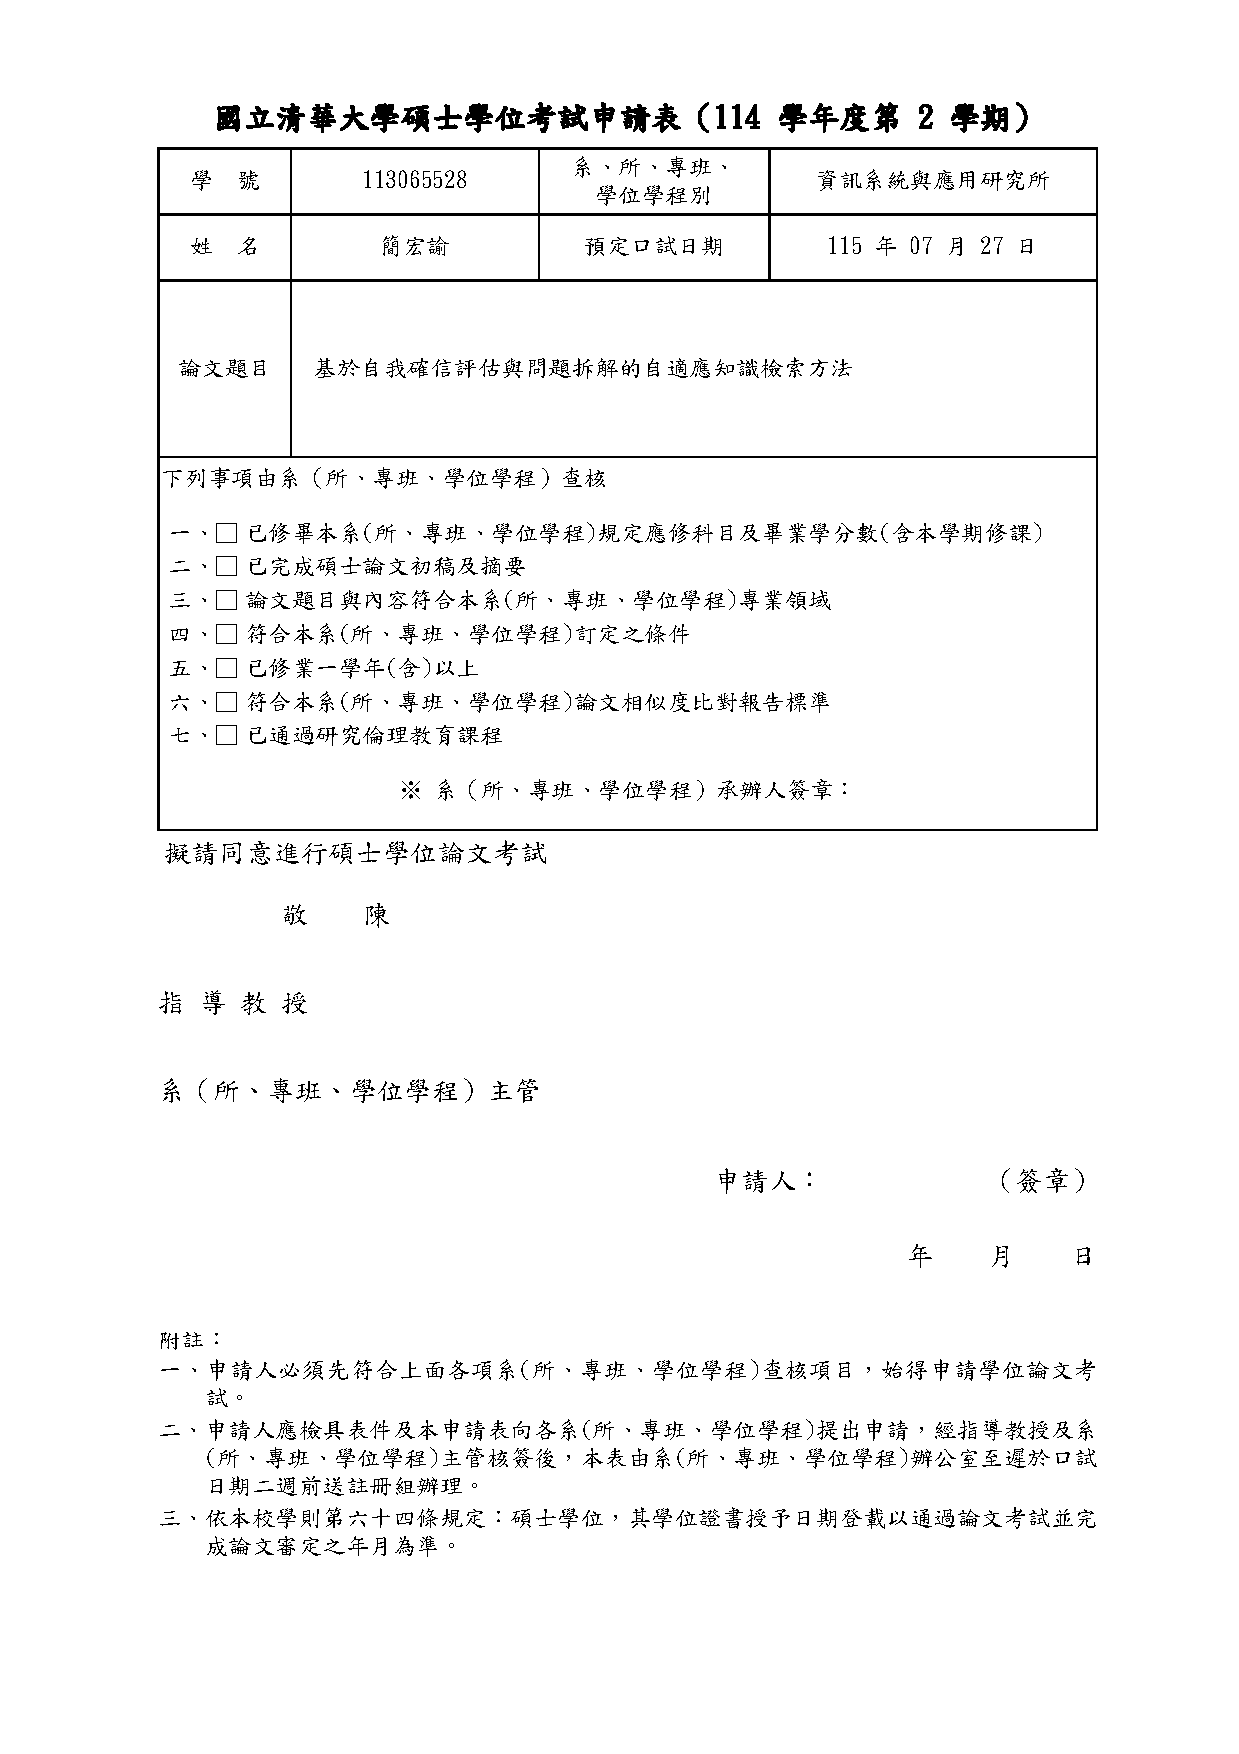
\includepdf[pages=1, angle=0, fitpaper=true,
    keepaspectratio, pagecommand={{\thispagestyle{empty}}}]{./front/Advisor Approval Form.pdf}

%\cftaddtitleline{<ext>}{<kind>}{<text>}{<page>} intead of using \addcontentsline command  for without page numbering

       
\cftaddtitleline{toc}{chapter}{指導教授推薦書}{}


\includepdf[pages=1, angle=0, fitpaper=true,
       keepaspectratio, pagecommand={{\thispagestyle{empty}}},offset=-0.0cm 0.0cm]{./front/Thesis Review Form.pdf} % offset=+right +up

\cftaddtitleline{toc}{chapter}{考試委員審定書}{}

\frontmatter %Use for book class 

%\pagenumbering{roman} %set lowercase Roman numerals for page numbers if set report class

%%% Necessary 中文摘要%%%

\chapter*{Abstract}
\addcontentsline{toc}{chapter}{Abstract}
This thesis proposes SEEK (Self-certainty Evaluated Evidence-gated Knowledge-retrieval), a lightweight adaptive Retrieval-Augmented Generation (RAG) framework for open-domain question answering. Fixed retrieval can distract simple questions and miss intermediate entities needed by multi-hop questions. Adaptive RAG must decide both whether to retrieve and whether decomposition can expose evidence without discarding global context. Existing approaches rely on coarse routing, imperfect uncertainty signals, or costly learned policies.

SEEK couples step-level retrieval gating with late path selection. A compact decomposer receives one LoRA supervised fine-tuning pass on 12,000 examples from MuSiQue, 2WikiMultihopQA, and PopQA. At inference, SEEK retains direct and decomposed candidates, gates sub-question retrieval with tail-leakage surprisal, adds original-question evidence to decomposed contexts, and uses a training-free type-aware verifier. Decomposition thus remains reversible and routing inspectable.

Across four question-answering datasets under full-corpus Wikipedia retrieval, decomposition improves answer-containing retrieval on the three multi-hop datasets by 5.53--28.03 hit@5 points and leaves single-hop PopQA nearly unchanged at $-0.10$ points. The two answer paths solve different questions, leaving 2.9--6.0 EM of oracle routing headroom. At the accuracy-first threshold of 0.002305, the gate retrieves for 93.84\% of decomposed steps and matches the rounded macro EM of always retrieving while avoiding 6.16\% of retrieval calls. Tail-leakage surprisal is nevertheless not a correctness guarantee, and retrieval gaps account for 47.6--70.1 percent of decomposition-path errors on the multi-hop datasets. Overall, SEEK reaches 41.88 EM and 48.90 F1 on average, compared with 38.45 EM and 45.75 F1 for DeepRAG. The analysis identifies retrieval coverage, bridge-answer propagation, and path selection as the main remaining bottlenecks.

\bigskip
\noindent\textbf{Keywords:} Retrieval-Augmented Generation, Adaptive Retrieval, Multi-hop Question Answering, Tail-Leakage Surprisal, Verifier Routing, Large Language Models
     % Insert English Abstract
\setcounter{page}{1}  %set page begins with i
\clearpage

\chapter*{摘要}
\addcontentsline{toc}{chapter}{摘要}
本研究提出 SEER (Sub-question Entropy-driven Efficient Retrieval)，一個基於子問題層級的自適應檢索增強生成 (Retrieval-Augmented Generation, RAG) 框架。現有 RAG 系統在面對不同複雜度的查詢時，往往採用一體適用的檢索策略：對簡單問題進行不必要的檢索會引入雜訊並增加成本；對複雜的多跳推理問題僅進行單次檢索則經常導致答案不完整或錯誤。

近期的自適應 RAG 方法雖試圖解決此問題，但其決策粒度往往不適切：問題層級的路由過於粗糙，無法在推理過程中即時調整；詞元 (token) 層級的偵測則過於嘈雜。雖有方法採用子問題層級的決策 (如 DeepRAG)，但仰賴二元樹搜尋、SFT 與 DPO 等繁複訓練流程，犧牲了可攜性與可解釋性。

本研究的核心想法是：將複雜問題分解為原子化子問題後，針對每個子問題答案中的「首實體跨度 (first-entity span)」計算熵值，作為模型自信度的指標，再以此決定是否觸發檢索。SEER 包含三階段：(1) 資料建構，整合 MuSiQue、HotpotQA 與 2WikiMultiHopQA 資料集並進行品質過濾；(2) 以 SFT 訓練輕量化分解器；(3) 訓練無關的熵閾值門控機制。我們預期 SEER 在多跳問答基準上能達到與 DeepRAG 相當的 Exact Match 表現，同時顯著降低訓練成本並提升可解釋性。

\bigskip
\noindent\textbf{關鍵字：}檢索增強生成、自適應檢索、多跳問答、熵、子問題分解、大型語言模型
    % 插入中文摘要於此 Insert Chinese Abstract

\clearpage


\chapter*{Acknowledgements}
\addcontentsline{toc}{chapter}{Acknowledgements}
% 致謝 Acknowledgements — 請於此處填寫致謝內容。
% 建議感謝對象包括：指導教授、口試委員、實驗室同仁
% (Intelligent Knowledge Management Lab)、提供研究資源的單位、家人與朋友等。

I would like to express my sincere gratitude to my advisor for the guidance and support throughout this research. I also thank the members of the Intelligent Knowledge Management Lab at National Tsing Hua University, the thesis oral examination committee, and all those who provided computational resources and helpful discussions. Finally, I thank my family and friends for their continuous encouragement.
      % Acknowledgement
\clearpage

% generate Contents of Tables, lists of figures, tables, 

\tableofcontents
\addcontentsline{toc}{chapter}{Contents}
\clearpage

\listoffigures  % Insert list of figures
\addcontentsline{toc}{chapter}{List of Figures}
\clearpage

\listoftables  % Insert list of tables
\addcontentsline{toc}{chapter}{List of Tables}
\clearpage

%Nomenclature (optional). List unfamiliar terms, symbols, acronyms and their meanings.
% List of Abbreviations — 縮寫對照表
% 使用 \nomenclature{縮寫}{全名} 新增條目，編譯後會自動排序列出。

\nomenclature{RAG}{Retrieval-Augmented Generation}
\nomenclature{SEEK}{Self-certainty Evaluated Entropy-gated Knowledge-retrieval}
\nomenclature{LLM}{Large Language Model}
\nomenclature{LM}{Language Model}
\nomenclature{QA}{Question Answering}
\nomenclature{SFT}{Supervised Fine-Tuning}
\nomenclature{DPO}{Direct Preference Optimization}
\nomenclature{MDP}{Markov Decision Process}
\nomenclature{EM}{Exact Match}
\nomenclature{AUROC}{Area Under the Receiver Operating Characteristic Curve}
\nomenclature{PPL}{Perplexity}
\nomenclature{CoT}{Chain-of-Thought}
\nomenclature{FLARE}{Forward-Looking Active REtrieval augmented generation}
\nomenclature{NTHU}{National Tsing Hua University}

\renewcommand{\nomname}{List of Abbreviations}
\printnomenclature
    % if needed Nomenclature
\addcontentsline{toc}{chapter}{Nomenclature}
\clearpage

% Contents of Thesis

\mainmatter  %for book class only
%\pagenumbering{arabic} % already default for book class, Arabic/Indic page numbers, needed for article class

\pagestyle{plain} %This is the default style for most document classes. It places the page number centered in the footer, with an empty header.
\chapter{Introduction}
\label{ch:introduction}

\section{Background and Motivation}

Large language models (LLMs) have become strong general-purpose generators, but the knowledge encoded in their parameters is necessarily incomplete and fixed at training time. When a question concerns recent events, long-tail entities, or information outside the training distribution, an LLM may still produce a fluent answer even when the underlying facts are unsupported. This behaviour limits the reliability of LLMs in knowledge-intensive applications~\cite{hallucination_survey}.

Retrieval-Augmented Generation (RAG) mitigates this problem by retrieving external passages and conditioning generation on the resulting evidence~\cite{rag_survey}. Because the evidence source can be updated independently of the language model, RAG provides a practical way to extend the model's accessible knowledge without repeated model training. A fixed retrieval strategy, however, is not equally suitable for every question. For a simple question that the model can already answer, irrelevant passages can introduce distractors and additional latency. For a complex multi-hop question, one retrieval query based on the original question may fail to expose the intermediate entity needed to locate the next supporting passage~\cite{ren2023,ircot}.

Adaptive RAG addresses this mismatch by changing the retrieval strategy according to the question or the model's state. Existing approaches include question-level complexity and self-knowledge routers~\cite{adaptiverag,skr}, uncertainty-triggered retrieval during generation~\cite{flare,dragin}, and learned policies that decide retrieval actions at individual reasoning steps~\cite{selfrag,deeprag}. These approaches demonstrate that retrieval need is query-dependent, but each has a different limitation. A question-level route is decided before the intermediate reasoning states are known; uncertainty is an imperfect proxy for correctness; and a learned step-level policy can require additional trajectory construction, supervision, or preference optimisation.

Multi-hop question answering introduces a second decision that is closely coupled with retrieval: whether to decompose the question. Question decomposition can convert a compositional question into shorter sub-questions that expose bridge entities and form more precise retrieval queries~\cite{decomprc,break_qdmr}. Nevertheless, decomposition is not uniformly reliable. An incorrect intermediate answer can misdirect later queries, while a short sub-question can omit comparison targets, entity pairs, or disambiguating conditions from the original question. Forcing every question through a decomposed path may therefore discard useful global context even when the retrieved passages themselves are relevant.

This thesis consequently frames adaptive RAG as a \emph{decomposition-routing problem}. A system should decide at two levels: whether each decomposed sub-question requires external evidence, and whether the final answer should be taken from the original-question path or the decomposed reasoning path. Preserving both paths makes decomposition a candidate strategy rather than an irreversible early commitment. This perspective motivates SEEK (Self-certainty Evaluated Evidence-gated Knowledge-retrieval), a lightweight framework that trains a compact decomposer but keeps retrieval gating and final path verification transparent and training-free.

Accordingly, this thesis investigates whether competitive adaptive RAG can be achieved with lightweight decomposition training and interpretable inference-time routing, without learning a separate retrieval policy. Its objectives are to produce structurally reliable and executable sub-questions, examine both the value and the limits of token-level self-certainty for sub-question retrieval, design a context-preserving dual-path procedure with transparent final verification, and evaluate the resulting framework across single-hop and multi-hop open-domain question answering in terms of accuracy, retrieval behaviour, offline adaptation cost, and failure modes.

\section{Research Contributions}

Our contributions are as follows:

\begin{enumerate}
    \item \textbf{Dual-path decomposition routing.} This thesis treats adaptive RAG as a choice between an original-question answer path and a decomposed answer path, rather than only a retrieve-or-skip decision. SEEK keeps both candidates until a final verification step, so decomposition becomes a reversible strategy instead of an early commitment. The two paths prove complementary: in the final traces, an oracle choice between them would add a further 2.9 to 6.0 EM, and the training-free verifier recovers part of this headroom.

    \item \textbf{A low-cost executable decomposer.} The decomposer is adapted in a single supervised LoRA~\cite{lora} pass on 12{,}000 examples and emits KG-style \texttt{entity >> relation} sub-questions with explicit \texttt{\#N} dependencies that resolve into directly executable retrieval queries. Keeping original-question evidence available at every decomposed step preserves global context that short sub-questions may omit, without changing the decomposer or training another retriever.

    \item \textbf{A simple confidence gate with a measured accuracy--retrieval trade-off.} Tail Leakage, computed from the probability mass the model keeps within its own top-five token candidates during a single greedy pass, gates sub-question retrieval. It captures a simple pattern: answers are more likely to be wrong when more probability falls outside these leading candidates. The score therefore measures only the total leaked mass, regardless of how probability is divided within the top five or distributed across the tail.

    \item \textbf{Training-free late verification.} A deterministic verifier reads direct-answer confidence, decomposition stability, and answer-type compatibility, and selects the final path so that every routing decision remains inspectable. The oracle comparison quantifies the remaining selection headroom without attributing candidate-generation gains to the verifier itself.
\end{enumerate}

\chapter{Related Work}
\label{ch:related}

\section{Adaptive RAG}
\label{sec:adaptive-rag}

Retrieval-Augmented Generation (RAG)~\cite{rag_survey} augments a parametric language model with a non-parametric retriever, allowing the model to condition its generation on external evidence rather than relying only on parameters learned during pretraining. A typical RAG pipeline can be described as five stages:

\begin{enumerate}
    \item \textbf{Indexing.} The source corpus is segmented into passages, and each passage is stored in a form that supports retrieval, such as sparse lexical indexes or dense vector representations.
    \item \textbf{Query manipulation.} The input question may be rewritten, expanded, normalised, or decomposed so that the retriever can better match it with relevant evidence.
    \item \textbf{Retrieval.} The system selects candidate passages from the indexed corpus, commonly using sparse lexical matching, dense vector similarity, or a hybrid retrieval strategy.
    \item \textbf{Post-retrieval processing.} The initially retrieved passages may be filtered, reranked, compressed, or otherwise refined before they are passed to the generator.
    \item \textbf{Generation.} The language model conditions on the selected evidence and produces the final answer, ideally grounding its output in the retrieved passages.
\end{enumerate}

This retrieve-then-generate paradigm is now widely used to make language model outputs more factual in question answering, explanation writing, and other knowledge-intensive tasks. Its central advantage is that factual evidence can be updated externally without retraining the language model. For multi-hop question answering, however, the quality of the retrieved evidence depends strongly on the query that is issued at each step: a single original question may not contain the intermediate entity needed to retrieve the next supporting passage.

This fixed retrieval assumption creates two well-documented failure modes:

\begin{itemize}
    \item \textbf{Noise injection on easy queries.} For questions the model already knows (e.g.\ ``Who wrote \emph{Hamlet}?''), retrieved passages introduce distractor entities that can override correct parametric knowledge~\cite{hallucination_survey}.
    \item \textbf{Insufficient evidence on hard queries.} For multi-hop questions, a single retrieval pass rarely surfaces all bridging entities, leading to incomplete or compositionally wrong answers~\cite{ircot}.
\end{itemize}

These two failure modes motivate adaptive retrieval: deciding \textbf{when} retrieval is \mbox{useful}, \textbf{how much} evidence to fetch, and what signal should determine the gate.

Adaptive RAG methods decide whether and how much to retrieve for each query or reasoning step. They can be characterised along three axes: decision granularity, gating signal, and training cost. Decision granularity ranges from question-level routing to sentence-, token-, or sub-question-level decisions, while training cost ranges from training-free methods to supervised fine-tuning, reinforcement learning, or preference optimisation. Since the gating signal is the most consequential axis for SEEK, we organise existing methods into three families: classifier-based gating, confidence-based gating, and reasoning-step decision methods.

\paragraph{Classifier-based gating.}

The first family trains a dedicated discriminator that inspects the query and emits a retrieval decision.

\textbf{Adaptive-RAG}~\cite{adaptiverag} routes each incoming query to one of three retrieval strategies according to its predicted complexity. Easy questions are answered without retrieval, medium-complexity questions use a single retrieval step, and complex questions are routed to a multi-step retrieve-and-reason pipeline such as \textbf{IRCoT}~\cite{ircot}. The router is a T5-Large classifier trained with automatically derived labels. Each training question is assigned to the cheapest strategy that still produces the correct answer, so the classifier learns a cost-aware mapping from question complexity to retrieval depth. This design reduces unnecessary retrieval compared with always using a multi-step pipeline. However, the decision is made only once at the beginning of the query. As a result, the system cannot react to uncertainty that appears during intermediate reasoning, and its routing labels remain coarse: questions with different numbers of reasoning hops may still be assigned to the same multi-step category.

\textbf{SKR}~\cite{skr} approaches adaptive retrieval from the perspective of self-knowledge. Instead of predicting general question complexity, SKR estimates whether the language model is likely to know the answer from its own parametric memory. If the question is judged as known, the model answers directly; if it is judged as unknown, external retrieval is invoked. This judgement can be implemented with a trained classifier or with memory-based self-knowledge strategies. In the classifier setting, SKR is a binary retrieval gate: it decides whether to retrieve, but does not distinguish between single-step and multi-step retrieval. Therefore, compared with Adaptive-RAG, SKR gives a more direct estimate of whether retrieval is needed, but it still commits to a question-level decision before reasoning begins.


\paragraph{Confidence- and uncertainty-based gating.}

The second family replaces an external router with uncertainty signals observed during generation. These methods are often training-free, since the retrieval decision is derived from token probabilities, entropy, \mbox{attention} patterns, or internal model states rather than from an additional trained classifier.

\textbf{FLARE}~\cite{flare} moves the retrieval decision from the question level to the generation level. At each step, it first drafts a tentative next sentence and checks whether the sentence contains low-confidence tokens. If the confidence falls below a threshold, the tentative sentence is used to formulate a retrieval query, and the model regenerates the sentence with the retrieved evidence. This design allows retrieval to occur only when the model appears uncertain during generation. However, token probability is only an indirect proxy for factual uncertainty. A low-probability token may reflect lexical variation rather than missing knowledge, and sentence-level regeneration may not align well with multi-hop reasoning, where the natural decision unit is often a sub-question.

\textbf{DRAGIN}~\cite{dragin} further refines dynamic retrieval by considering both when to retrieve and what to retrieve. Its \emph{Real-time Information Need Detection}(RIND) module estimates whether the current generation state requires external evidence, while its \emph{Query Formulation based on Self-attention}(QFS) module constructs retrieval queries from salient \mbox{context} tokens instead of relying only on the most recent sentence. Compared with FLARE, DRAGIN provides a more context-aware retrieval trigger and query formulation strategy. Nevertheless, its decision is still made at the token-generation level, which can be mismatched with explicit sub-question reasoning, and it introduces additional overhead from attention-based query construction.

\textbf{SeaKR}~\cite{seakr} estimates retrieval need from the model's internal states rather than from output probabilities alone. It activates retrieval when the model exhibits high self-aware uncertainty and reranks retrieved passages according to how much they reduce that uncertainty. This makes the retrieval signal more closely tied to the model's internal generation dynamics than token-level probability alone. However, the signal is still an estimate of \mbox{uncertainty} rather than a direct measure of answer correctness. A model may be uncertain for reasons unrelated to missing external knowledge, and retrieval may not necessarily improve the answer even when uncertainty is high.

\textbf{TARG}~\cite{targ} studies adaptive retrieval as a training-free, single-shot decision. It generates a short no-context draft and computes uncertainty from the prefix logits to decide whether retrieval should be invoked. In addition to entropy, TARG considers a top-1/top-2 logit-margin signal and a small-sample variance signal. Its main strength is that it \mbox{provides} a lightweight retrieval gate without training an auxiliary classifier or modifying the language model. However, its evaluation mainly focuses on open-domain factoid QA settings, where each question is typically answered with a single retrieval decision. Its behaviour in multi-hop QA or decomposition-based retrieval settings therefore remains less explored.

Across this family, uncertainty provides a useful and interpretable signal for adaptive retrieval, but it remains an imperfect proxy. Low uncertainty does not guarantee a correct answer, and high uncertainty does not always indicate that retrieval will help. SEEK addresses this limitation by using entropy as a sub-question retrieval signal and as one component of a late verifier, rather than treating it as a single hard router for the entire question.

\paragraph{Learned retrieval-policy methods.}

The third family does not rely on a fixed classifier or a hand-set uncertainty threshold. Instead, it learns retrieval decisions as part of the model's reasoning or generation process.

\textbf{Self-RAG}~\cite{selfrag} trains the language model to generate special reflection tokens that control retrieval and evaluate retrieved passages. For example, the model can emit \texttt{[Retrieve]} to decide whether external evidence is needed, and then use additional tokens to judge whether a passage is relevant, supportive, or useful. This design makes retrieval part of generation itself, rather than a separate preprocessing step. However, it requires fine-tuning on reflection-token supervision and a custom decoding procedure that interleaves normal text generation with retrieval-related decisions.

\textbf{DeepRAG}~\cite{deeprag} formulates retrieval-augmented reasoning as a step-by-step decision process. At each sub-query, the model chooses between answering from parametric memory and issuing a retrieval call. Its training procedure first uses binary tree search to explore both choices for each sub-query, and then applies preference-based calibration to learn which reasoning traces should be preferred. This gives DeepRAG strong sub-question-level retrieval control, but the cost is substantial. Tree-search rollout becomes expensive as the number of reasoning steps grows, preference pairs must be carefully constructed, and the final retrieval policy is learned implicitly rather than exposed as an interpretable score.

A related line of work studies retrieval cost more directly. \textbf{Fast-or-Better}~\cite{fastorbetter} treats the number of retrieved passages or retrieval calls as a controllable trade-off between latency and accuracy, rather than assuming one fixed operating point. This view reinforces an important point for adaptive RAG: retrieval should be evaluated not only by accuracy, but also by the cost required to obtain that accuracy.

SEEK is closest in spirit to DeepRAG because both methods make retrieval decisions at the sub-question level. The key difference is that SEEK avoids tree search and preference optimisation. It uses a single supervised decomposer and replaces the learned retrieval policy with a training-free verifier based on entropy, decomposition stability, answer type, and candidate agreement.

Table~\ref{tab:related-work} summarises the key differences between SEEK and existing adaptive RAG methods along the three axes introduced above. SEEK occupies the under-explored region of \emph{late verifier-based routing with interpretable, training-free signals}: only a single SFT pass is needed for the decomposer, and the final route is decided by transparent query-level diagnostics rather than a learned policy.

\begin{table}[h]
    \centering
    \caption[Comparison of Adaptive RAG Methods]{Comparison of adaptive RAG methods along granularity, gating signal, interpretability, training cost, and decision unit.}
    \label{tab:related-work}
    \setlength{\tabcolsep}{6pt}
\begin{tabular}{ l c c c c c }
        \toprule
        Method & Decomposer & Gating Signal & Interpretable & Training Cost & Granularity \\
        \midrule
        Adaptive-RAG~\cite{adaptiverag} & None       & Query classifier            & Partial & Low (T5-Large) & Question \\
        FLARE~\cite{flare}              & None       & Token probability           & Yes     & None           & Sentence \\
        Self-RAG~\cite{selfrag}         & None       & Reflection tokens           & Partial & High (distill) & Span \\
        DRAGIN~\cite{dragin}            & None       & Entropy + attention         & Yes     & None           & Token \\
        SKR~\cite{skr}                  & None       & Binary self-knowledge       & Partial & Low            & Question \\
        SeaKR~\cite{seakr}              & None       & Hidden-state variance       & No      & None           & Sentence \\
        TARG~\cite{targ}                & None       & Prefix uncertainty          & Yes     & None           & Question \\
        DeepRAG~\cite{deeprag}          & SFT        & Learned policy (SFT+DPO)    & No      & High           & Sub-Q \\
        \textbf{SEEK (Ours)}            & SFT        & Entropy-aware verifier       & \textbf{Yes} & \textbf{Low} (SFT only) & \textbf{Sub-Q + query} \\
        \bottomrule
    \end{tabular}
\end{table}

\section{Reasoning and Knowledge Boundaries in RAG}
\label{sec:reasoning-rag}
\label{sec:knowledge-boundary}

A parallel thread focuses on \emph{how} to retrieve and reason once retrieval is deemed necessary, independent of the gate.

The foundational technique is \textbf{IRCoT}~\cite{ircot}, which interleaves chain-of-thought reasoning with retrieval: after each generated CoT sentence, the partial reasoning becomes the next query. IRCoT is the canonical “multi-step” implementation referenced by \textbf{Adaptive-RAG}~\cite{adaptiverag} and \textbf{DeepRAG}~\cite{deeprag}, but its retrieval count grows linearly in the CoT length, regardless of whether intermediate steps are factually difficult. Question decomposition provides a complementary way to structure multi-hop QA. Rather than retrieving after each free-form reasoning sentence, decomposition-based methods explicitly split a complex question into simpler sub-questions that can be answered independently or sequentially. Early systems such as \textbf{DecompRC}~\cite{decomprc}  show that compositional questions can be reduced to single-hop reading-comprehension steps, while \textbf{BREAK/QDMR}~\cite{break_qdmr} formalises decomposition as an ordered sequence of natural-language operations required to answer the original question. SEEK inherits this decomposition paradigm, but uses it primarily as an inspectable reasoning path: it preserves the original-question context for decomposed steps, evaluates whether the generated sub-questions are useful, and verifies whether the direct or decomposed answer should be trusted.

More recent work synthesises reasoning data to internalise the retrieve-and-reason loop. \textbf{Auto-RAG}~\cite{autorag} autonomously synthesises multi-turn retrieval--reasoning trajectories and fine-tunes on them, so that the model plans its own retrieval steps without hand-crafted prompts. \textbf{Search-o1}~\cite{searcho1} embeds retrieval inside a large reasoning model in an agentic loop, augmenting o1-style long-chain reasoning with on-demand search and a document-reasoning module that distils retrieved passages before they re-enter the chain. \textbf{AirRAG}~\cite{airrag} activates the model's intrinsic reasoning by combining Monte Carlo Tree Search with self-consistency to explore alternative solution paths. These methods substantially strengthen the reasoning side of RAG, but --- like DeepRAG --- they rely on heavy data synthesis or search-time expansion; SEEK instead keeps the reasoning component a single lightweight SFT decomposer and concentrates its novelty in training-free verification.

Every adaptive method above ultimately rests on a model's ability to recognise its own \emph{knowledge boundary} --- the line between what it reliably knows and what it must look up. A dedicated line of work studies this capacity directly, and we group it into three strands: \emph{self-knowledge elicitation}, \emph{uncertainty estimation}, and the \emph{interaction between the knowledge boundary and retrieval}.

\paragraph{Self-knowledge and its calibration.} A first strand asks whether a model can introspect on what it knows. Kadavath et al.~\cite{kadavath2022} show that LLMs are, to a useful degree, calibrated: a model can be prompted to predict the probability \texttt{P(True)} that its own answer is correct, and these self-judgements correlate with actual accuracy --- though calibration degrades on out-of-distribution and adversarial questions. Yin et al.~\cite{yin2023} construct a ``SelfAware'' benchmark of answerable and unanswerable questions and find that LLMs only partially ``know what they don't know'': self-knowledge can be elicited but lags well behind human performance. From the supervised side, Kapoor et al.~\cite{kapoor2024} argue that models ``must be taught to know what they don't know'', demonstrating that lightweight calibration-tuning or probing substantially sharpens a model's estimate of its own uncertainty. Yin et al.~\cite{yin2024} formalise the notion of a knowledge boundary itself, proposing to benchmark a model by probing the frontier of its reliable knowledge rather than by aggregate accuracy alone.

\paragraph{Uncertainty estimation as a boundary signal.} A second strand asks how to \emph{measure} the boundary at inference time. Beyond retrieval-specific methods, recent work on LLM uncertainty quantification compares several confidence estimators for answer correctness, including token entropy, maximum softmax probability, margin-based scores, verbalised confidence, and response consistency~\cite{maqa}. These studies suggest that no single confidence signal is universally reliable across tasks and models. This motivates evaluating whether entropy is sufficient in SEEK's QA setting, or whether a margin-based signal provides a more discriminative retrieval gate.

Semantic entropy further shows why token-level uncertainty can be limited for natural-language answers: different surface forms may express the same meaning, so uncertainty over token sequences does not always correspond to uncertainty over answers. Kuhn et al.~\cite{semanticuncertainty} introduce \emph{semantic entropy}, which clusters multiple sampled answers by meaning before computing entropy, so that paraphrases of one correct answer do not register as uncertainty; Farquhar et al.~\cite{semanticentropy} scale this idea and show in \emph{Nature} that semantic entropy reliably detects confabulations across QA and biography generation. This observation is important for SEEK because exact QA answers often involve aliases, entity variants, and short spans. We therefore treat token entropy as a cheap diagnostic signal rather than as a correctness guarantee.

\paragraph{The boundary under retrieval.} A third strand studies the boundary specifically in the RAG setting. Ren et al.~\cite{ren2023} show that retrieval augmentation not only injects evidence but also \emph{reshapes} the boundary: relevant passages let a model answer questions it could not before, while irrelevant or distracting passages can push a previously-correct answer over the boundary into error --- precisely the ``noise injection on easy queries'' failure mode of \S\ref{sec:adaptive-rag}. This makes a per-step boundary estimate, rather than a one-shot query-level one, essential when retrieval and reasoning are interleaved.

These three strands form the conceptual foundation of SEEK. The failure modes of \S\ref{sec:adaptive-rag} --- spurious retrieval on easy queries, missing retrieval on hard ones, and confident hallucination under a hard entropy threshold --- are all symptoms of a poorly localised knowledge boundary. Where confidence-based methods read a single uncertainty proxy and policy-based methods bury the boundary inside a learned policy, SEEK makes the boundary inspectable through a late verifier: entropy, decomposition stability, and answer agreement jointly decide whether the direct or decomposed path should be trusted.

\section{Evaluation Datasets}
\label{sec:evaluation-datasets}

The evaluation of adaptive RAG hinges on datasets that span both single-hop and multi-hop complexity. This thesis uses HotpotQA, 2WikiMultihopQA, MuSiQue, and PopQA to cover both multi-hop reasoning and single-hop factual recall.

\paragraph{HotpotQA.}

HotpotQA~\cite{hotpotqa} is the canonical multi-hop QA benchmark, containing 113K Wikipedia-based questions requiring 2-hop reasoning. Each example provides (a) the question, (b) the gold answer, (c) two gold-supporting paragraphs out of 10 distractors (in the \texttt{distractor} setting), and (d) sentence-level supporting facts. Questions fall into two compositional patterns: \emph{bridge} (the answer to sub-question 1 is the subject of sub-question 2) and \emph{comparison} (two entities are compared along a shared attribute). HotpotQA is a primary training source for DeepRAG and a standard evaluation set for nearly all adaptive RAG papers.

\paragraph{2WikiMultihopQA.}

2WikiMultihopQA~\cite{twowiki} constructs 192K multi-hop questions by leveraging Wikidata knowledge-graph paths, ensuring each question requires traversal of an explicit reasoning chain. It includes four question types (comparison, inference, compositional, and bridge-comparison) and provides KG-triple annotations alongside textual evidence. Compared to HotpotQA, 2WikiMultihopQA exhibits less surface-form leakage between the question and the supporting passages, making it a more reliable test of compositional reasoning.

\paragraph{MuSiQue.}

MuSiQue (\textbf{Mu}ltihop questions via \textbf{Si}ngle-hop \textbf{Que}stions)~\cite{musique} addresses two pathologies of earlier datasets: (i) shortcut answers via single-hop reasoning, and (ii) weak distractor selection. MuSiQue is built by composing 2--4 single-hop questions into chains using strict connectivity criteria, yielding 25K questions of 2-hop, 3-hop, and 4-hop varieties. Importantly, MuSiQue provides the \emph{decomposed} sub-questions as supervision, which makes it a natural training source for decomposer models such as the one used in SEEK. Its high distractor difficulty makes it the hardest of the four datasets in this thesis.

\paragraph{PopQA.}

PopQA~\cite{popqa} is a \emph{single-hop} entity-centric QA dataset of 14K questions, each derived from a Wikidata subject--property--object triple. Critically, PopQA tags each entity with its \emph{popularity} (measured by monthly Wikipedia page views), enabling stratified evaluation of factual recall on long-tail entities. Despite being single-hop, PopQA exposes the over-decomposition failure mode of decomposer-based pipelines: trained on multi-hop data, a decomposer may emit two-step plans even when one step suffices, harming both EM and efficiency.

\paragraph{Single-hop open-domain QA.}

For completeness, prior adaptive-RAG papers also evaluate on \textbf{Natural Questions (NQ)}~\cite{nq}, \textbf{TriviaQA}~\cite{triviaqa}, and \textbf{SQuAD}~\cite{squad}. These are single-hop datasets whose answers typically exist in a single Wikipedia paragraph, and they primarily test whether an adaptive method can correctly \emph{skip} retrieval rather than orchestrate it. This thesis follows the DeepRAG protocol of evaluating on PopQA as the representative single-hop test set.

\chapter{Methodology}
\label{ch:method}

This chapter presents \textbf{SEEK} (\textbf{S}elf-certainty \textbf{E}valuated \textbf{E}vidence-gated \textbf{K}nowledge-retrieval), a lightweight adaptive RAG framework that treats question decomposition as a routing problem. SEEK runs both a direct path and a decomposition path, preserves original-question evidence inside decomposed steps, and chooses between the candidate answers using a training-free verifier. The design follows the view that adaptive RAG is more than a retrieve-or-skip problem: a question may need to be answered directly, decomposed into sharper retrieval queries, or repaired with original-question context after decomposition.

\section{Overview}
\label{sec:overview}

Given a question $q$ and an open-domain retrieval corpus $\mathcal{P}$, SEEK produces a final answer $\hat{a}$ through two candidate-generation paths followed by a verifier. Figure~\ref{fig:pipeline} shows the overall pipeline:

\begin{enumerate}
    \item \textbf{Direct path.} The answerer directly answers the original question $q$ with BM25 evidence retrieved from $\mathcal{P}$, producing a direct candidate $a^{\mathrm{dir}}$ and a token-level confidence score $\sigma^{\mathrm{dir}}$ over the generated answer span.
    \item \textbf{Decomposition path.} The decomposer $\mathcal{D}_\theta$ maps $q$ to ordered sub-questions $\{s_1, \ldots, s_n\}$. Each sub-question is answered sequentially, with placeholder substitution, confidence probing, conditional retrieval, original-question evidence union, and a final synthesis step that produces $a^{\mathrm{dec}}$.
    \item \textbf{Training-free verifier.} A deterministic verifier compares $a^{\mathrm{dir}}$ and $a^{\mathrm{dec}}$ using direct-answer confidence, decomposition stability, and answer-type compatibility. It returns either $a^{\mathrm{dir}}$ or $a^{\mathrm{dec}}$ as $\hat{a}$.
\end{enumerate}

\begin{figure}[htbp]
    \centering
    \makebox[\linewidth][c]{\includegraphics[width=1.3\linewidth]{Thesis_overflow.pdf}}
    \caption[SEEK Pipeline]{Overview of SEEK. Stage 1 constructs 12K gold decomposition examples from MuSiQue, 2WikiMultihopQA, and PopQA; Stage 2 trains the LoRA decomposer on this corpus; Stage 3 runs dual-path inference, where the direct path answers the original question with retrieved evidence and the decomposition path answers sub-questions sequentially with confidence-gated retrieval and answer propagation, and a training-free verifier selects the final answer.}
    \label{fig:pipeline}
\end{figure}

\section{Problem Formulation}

We study open-domain question answering: given a natural-language question $q$ and a passage corpus $\mathcal{P}$, the system outputs a short answer span $\hat{a}$, which is evaluated against gold answers by exact match and F1. The questions of interest are often multi-hop, so a single retrieval with the original question may not surface all the required evidence. Let $\mathcal{M}_\theta$ be a pretrained language model, $r(q, \mathcal{P}, k)$ a BM25 retriever over an open-domain corpus $\mathcal{P}$, and $\mathcal{D}_\theta(q)$ a decomposer that emits sub-questions. A conventional retrieve-then-read system produces one answer from one path. SEEK instead constructs two candidates. The direct candidate answers the original question with retrieved evidence:

\[
    a^{\mathrm{dir}} = \mathcal{M}_\theta(q, r(q, \mathcal{P}, k)).
\]

The decomposition candidate first maps the question to an ordered list of sub-questions,

\[
    \{s_1, \ldots, s_n\}=\mathcal{D}_\theta(q),
\]

then answers each sub-question $s_i$ in order to obtain $a_i$, and finally synthesises the pairs into an answer span:

\[
    a^{\mathrm{dec}} = \mathrm{Synth}\left(q, \{(s_i, a_i)\}_{i=1}^{n}\right).
\]

Here $\mathrm{Synth}$ is not a string-level merge but a final generation pass of the base model $\mathcal{M}_\theta$: it reads $q$ together with all pairs $(s_i, a_i)$ and generates the final answer span under the prompt rules described in Section~\ref{sec:gate}.

The final decision is a verifier $v$:

\[
    \hat{a}=v\left(q, a^{\mathrm{dir}}, a^{\mathrm{dec}}, z^{\mathrm{dir}}, z^{\mathrm{dec}}\right),
\]

where $z^{\mathrm{dir}}$ and $z^{\mathrm{dec}}$ are inference-time diagnostic signals such as confidence scores, unresolved placeholders, and whether $a^{\mathrm{dir}}$ and $a^{\mathrm{dec}}$ are the same answer after normalisation. The verifier is a transparent rule set designed to approximate the oracle choice between direct and decomposed reasoning.

\section{Sub-Question Decomposer}
\label{sec:decomposer}

The decomposer emits one sub-question per line, prefixed with \texttt{\#}$\langle i \rangle$\texttt{:}. Each sub-question is expressed as a compact knowledge-graph fragment:

\begin{center}
    \texttt{\#}$i$\texttt{: }$\langle$\emph{entity}$\rangle$\texttt{ >> }$\langle$\emph{relation}$\rangle$
\end{center}

When a sub-question depends on an earlier answer, the placeholder \texttt{\#}$j$ refers to the answer of step $j$. For example:

\begin{center}
\begin{tabular}{ll}
    \texttt{\#1: Inception >> director} & $\rightarrow$ $a_1$ = \texttt{Christopher Nolan}\\
    \texttt{\#2: \#1 >> place of birth} & $\rightarrow$ \texttt{Christopher Nolan >> place of birth}
\end{tabular}
\end{center}

At inference, placeholders are resolved sequentially: \texttt{\#1} stands for the answer text of step 1, not its index. Once step 1 returns $a_1$, \texttt{\#1} in $s_2$ is replaced by that answer before retrieval and answering, as shown in the example above. The KG-triple notation is compact, consistent across datasets, and aligned with Wikidata-style supervision in 2WikiMultihopQA and PopQA.

The fixed instruction used to prompt the decomposer is shown in Figure~\ref{fig:decomposer-prompt}.

\begin{figure}[H]
    \centering
    \vspace{-1.2\baselineskip}
    \includegraphics[width=0.82\textwidth,trim=145bp 500bp 107bp 210bp,clip]{prompt_Decomposer.pdf}
    \caption[Decomposer Prompt]{Fixed instruction prompt used by the decomposer.}
    \label{fig:decomposer-prompt}
\end{figure}

The prompt standardises the output format without imposing a fixed decomposition depth. As Table~\ref{tab:decomp-examples} illustrates, the same representation accommodates one-hop fact lookup, bridge reasoning, comparison, and longer compositional chains.

\begin{table}[htbp]
    \centering
    \caption[Decomposition Patterns by Dataset]{Representative decomposition patterns produced by the SEEK decomposer.}
    \label{tab:decomp-examples}

    \setlength{\tabcolsep}{6pt}
    \small
    \begin{tabular}{ l p{4cm} p{6cm} }
        \toprule
        Dataset & Question type & Decomposition \\
        \midrule
        PopQA & 1-hop fact lookup & \texttt{\#1: George Rankin >> occupation} \\
        \addlinespace
        HotpotQA & 2-hop bridge & \texttt{\#1: Film X >> director} \newline \texttt{\#2: \#1 >> nationality} \\
        \addlinespace
        2WikiMultihopQA & comparison & \texttt{\#1: A >> date of birth} \newline \texttt{\#2: B >> date of birth} \\
        \addlinespace
        MuSiQue & compositional chain & \texttt{\#1: X >> capital} \newline \texttt{\#2: \#1 >> mayor} \newline \texttt{\#3: \#2 >> party} \\
        \bottomrule
    \end{tabular}
\end{table}

\paragraph{Training.} Only the decomposer requires training; the answerer, synthesizer, and verifier are training-free. The decomposer is a LoRA~\cite{lora} adapter on Llama-3-8B-Instruct, trained on 12{,}000 examples drawn equally from MuSiQue gold sub-questions, 2WikiMultihopQA evidence-triple conversions, and PopQA one-step triples. Before the PopQA examples were sampled, all 1{,}000 evaluation question IDs were removed; the resulting 4{,}000 PopQA training questions have zero exact overlap with the evaluation questions. The PopQA component teaches the decomposer that a one-step plan is valid. This improves single-hop robustness, but Chapter~\ref{ch:results} shows that it also creates negative transfer on some multi-hop datasets; the verifier is introduced precisely because no single hard decomposition policy is optimal across all query types. At inference, the adapter is enabled for decomposition and sub-question answering, and disabled for final synthesis, where the base instruction model produces shorter and more stable spans.

\clearpage

\section{Token-Level Confidence Probe}
\label{sec:probe}

The fixed answer-only instruction used for both direct and sub-question answering is shown in Figure~\ref{fig:answer-prompt}.

\begin{figure}[H]
    \centering
    \vspace{-1.2\baselineskip}
    \includegraphics[width=0.82\textwidth,trim=126bp 389bp 126bp 382bp,clip]{prompt_Answer.pdf}
    \caption[Answer Prompt]{Answer-only prompt for direct and sub-question generation.}
    \label{fig:answer-prompt}
\end{figure}

During greedy decoding, SEEK records the softmax distribution $p_t=\mathrm{softmax}(\mathrm{logits}_t)$ for each generated token $t$. All confidence signals in SEEK are derived from these distributions: generation is a single greedy pass, so no resampling-based agreement is available, and no additional model is trained to judge confidence.

\paragraph{Two kinds of uncertainty.} The signal design starts from an observation about how correct and incorrect answers differ at the token level. When the model knows the answer, the probability mass concentrates on a few candidates, and the remaining competition is typically between surface variants of the same answer, such as aliases, casing, or formatting differences. When the model lacks the required knowledge, the mass instead disperses over many unrelated continuations, well beyond any small set of plausible candidates. What separates the two cases is not how evenly the leading candidates split the mass, but whether the mass stays inside a small candidate set at all.

\paragraph{Locating the signal with R\'enyi entropy.} Before committing to a particular functional form, SEEK first asks \emph{which region} of the next-token distribution carries the error-related information. R\'enyi entropy~\cite{renyi1961} offers a controlled instrument for this question, because it leaves the underlying probabilities untouched and changes only the relative emphasis given to high- and low-probability tokens:

\begin{equation}
    H_\alpha(p_t)=\frac{1}{1-\alpha}\log\sum_{v} p_t(v)^{\alpha},
    \qquad \alpha>0,\ \alpha\neq 1,
    \label{eq:renyi}
\end{equation}

which recovers Shannon entropy in the limit $\alpha\rightarrow 1$. For $\alpha>1$ the sum is dominated by the largest probabilities, so the measure mainly describes the shape of the head; for $\alpha<1$ small probabilities are amplified, so the measure becomes increasingly sensitive to the tail. This distinction is consequential for LLM next-token distributions: over a vocabulary of more than 128K tokens, the tail consists of tens of thousands of individually negligible probabilities, and Shannon entropy, which weights each token by its own probability, folds their combined effect together with the competition among a handful of leading candidates into a single number. Substituting R\'enyi variants for Shannon entropy inside the same maximum-token-entropy error detector evaluated in Section~\ref{sec:tail-leakage-analysis} isolates the effect of this reweighting while holding everything else fixed; Figure~\ref{fig:renyi-reweight} visualises the reweighting and the resulting detection quality. On the 2WikiMultihopQA direct-path trace, the head-sensitive setting $\alpha=2$ reaches an error-detection AUROC of 0.651, Shannon entropy ($\alpha\rightarrow 1$) reaches 0.671, and the tail-sensitive setting $\alpha=0.5$ improves to 0.716. Detection quality rises monotonically as emphasis moves from the head towards the tail, which is the first piece of evidence that the error-related signal resides in the low-probability region rather than among the leading candidates. R\'enyi entropy nevertheless still compresses the entire distribution into one number: it indicates that the tail matters, but cannot distinguish whether what matters is \emph{how much} total mass leaks into the tail or \emph{how} that mass is arranged within it. The remainder of this section separates the two.

\begin{figure}[htbp]
    \centering
    \includegraphics[width=\textwidth]{fig_renyi_reweight_auroc.pdf}
    \caption[R\'enyi Reweighting and Error Detection]{R\'enyi reweighting of a next-token distribution and its effect on error detection. Left three panels: the escort distribution $p_t(v)^{\alpha}/\sum_{w} p_t(w)^{\alpha}$ of one fixed next-token distribution under three orders $\alpha$; $\alpha=2$ concentrates emphasis on the head (orange), $\alpha\rightarrow 1$ recovers the Shannon weighting, and $\alpha=0.5$ amplifies the tail (blue). Right: error-detection AUROC of the corresponding maximum-token-entropy detector on the 2WikiMultihopQA direct-path trace rises monotonically as emphasis moves towards the tail.}
    \label{fig:renyi-reweight}
\end{figure}

\paragraph{Same entropy, different risk.} A minimal example shows why a single entropy value cannot make this separation. Figure~\ref{fig:same-entropy-risk} and Table~\ref{tab:same-entropy-example} construct two next-token distributions for an answer position at which the model chooses between the casing variants \texttt{PO} and \texttt{po} of the same answer. The two distributions share identical leading candidates and, by construction, the same Shannon entropy of approximately $1.83$ nats. They differ only in where the remaining probability sits: distribution A retains $0.90$ of its mass inside the five most probable tokens and leaks $10\%$ into a dispersed tail of twelve tokens, whereas distribution B retains only $0.80$ and leaks twice as much mass into a more concentrated tail of five tokens. Entropy cannot separate the two cases because it responds simultaneously to the amount of leaked mass and to how dispersed that mass is: a smaller but more dispersed tail and a larger but more concentrated one sum to the same entropy. For the retrieval decision, however, the relevant event is that twice as much probability has escaped the model's main candidate set, while the competition between the two leading candidates—surface variants of one answer—is benign in both cases. The leakage score introduced below reacts to exactly this difference: $-\log 0.90 = 0.105$ versus $-\log 0.80 = 0.223$, more than doubling where entropy does not move at all.

\begin{figure}[htbp]
    \centering
    \includegraphics[width=\textwidth]{fig_same_entropy_risk.pdf}
    \caption[Same Entropy, Different Risk]{The two constructed distributions of Table~\ref{tab:same-entropy-example}. The two leading candidates (orange) are identical and both distributions have a Shannon entropy of $1.83$ nats, yet distribution B leaks twice as much probability mass into the tail (blue). The leakage score $-\log m_t$ more than doubles while entropy does not move.}
    \label{fig:same-entropy-risk}
\end{figure}

\begin{table}[htbp]
    \centering
    \caption[Same Entropy, Different Risk]{Two constructed next-token distributions with identical leading candidates and equal Shannon entropy (natural logarithm) but different tail mass. The per-token leakage score $-\log m_t$ defined in Section~\ref{sec:probe} separates them, whereas entropy does not.}
    \label{tab:same-entropy-example}
    \small
    \begin{tabular}{lcc}
        \toprule
         & Distribution A & Distribution B \\
        \midrule
        rank 1: \texttt{PO} & 0.38 & 0.38 \\
        rank 2: \texttt{po} & 0.26 & 0.26 \\
        ranks 3--5 & 0.11 / 0.08 / 0.07 & 0.06 / 0.05 / 0.05 \\
        \midrule
        top-five retained mass & 0.90 & 0.80 \\
        tail mass & 0.10 (12 tokens $\times$ 0.83\%) & 0.20 (5 tokens $\times$ 4.0\%) \\
        Shannon entropy (nats) & 1.83 & 1.83 \\
        leakage score $-\log m_t$ & 0.105 & 0.223 \\
        \bottomrule
    \end{tabular}
\end{table}

\paragraph{Decomposing token entropy.} Token entropy is the usual way to measure this kind of uncertainty, but it mixes the leakage of probability mass out of the candidate set with effects that are unrelated to correctness. Let $V_5(p_t)$ denote the set of the five most probable tokens under $p_t$, and let

\begin{equation}
    m_t = \sum_{v\in V_5(p_t)} p_t(v)
    \label{eq:topk-mass}
\end{equation}

be the probability mass retained within these candidates; the mass $1-m_t$ that leaks into the rest of the vocabulary is the tail. For token entropy $H(p_t)=-\sum_v p_t(v)\log p_t(v)$, the chain rule gives three components:

\begin{equation}
    H(p_t)=H_{\mathrm{B}}(m_t)+m_t\,H(\hat{p}_t^{\,\mathrm{in}})+(1-m_t)\,H(\hat{p}_t^{\,\mathrm{out}}),
    \label{eq:entropy-chain}
\end{equation}

where $H_{\mathrm{B}}$ is the binary entropy of whether the next token falls inside the top five or in the tail, and $\hat{p}_t^{\,\mathrm{in}}$, $\hat{p}_t^{\,\mathrm{out}}$ are the renormalised distributions inside and outside the top-five set. Only the first term reflects whether mass leaks into the tail. The second term measures competition inside the top five, which for correct answers frequently comes from surface variants of the same answer, and the third term describes the composition of the tail, which carries little information about correctness. Mixing the three therefore makes entropy a weaker error signal than the leakage term alone. This decomposition is an identity, not an approximation: it does not introduce a new uncertainty measure, but makes it possible to test each source of uncertainty separately. Section~\ref{sec:tail-leakage-analysis} performs exactly this test and confirms the reading: scored in isolation over the same traces, the leakage term reaches a macro error-detection AUROC of 0.742, competition inside the top five reaches 0.712, and the composition of the tail reaches 0.502, barely above chance. What predicts errors is how much mass leaves the candidate set, not how the leaked mass is arranged once it has left; this also resolves the ambiguity that the R\'enyi probe left open.

\paragraph{Tail-leakage surprisal.} The confidence signal of SEEK retains only the top-five mass $m_t$ from this decomposition and transforms it into a monotonic leakage score, while discarding the two within-group entropy terms. Surprisal is the standard information-theoretic measure of how unexpected an event is: an event of probability $p$ carries surprisal $-\log p$. Applying it to the event that generation stays within the candidate set, and accumulating over the answer, gives

\begin{align}
    \mathrm{TL}_t
        &= -\log m_t, \label{eq:tl-token} \\
    \sigma^{\mathrm{tl}}
        &= \sum_{t\in\mathcal{T}} \mathrm{TL}_t
         = -\log \prod_{t\in\mathcal{T}} m_t , \label{eq:tail-leakage}
\end{align}

where $\mathcal{T}$ indexes the generated answer tokens, excluding EOS. $\mathrm{TL}_t$ is the surprisal of staying inside the candidate set at position $t$: it is near zero when the top five candidates retain almost all of the mass, and it grows as mass leaks into the tail.

The transform is deliberately \emph{not} the binary-entropy term $H_{\mathrm{B}}(m_t)$ of Equation~\eqref{eq:entropy-chain}. A risk score should satisfy a basic monotonicity requirement: the more probability leaves the candidate set, the higher the score, with no reversal at severe leakage. As Figure~\ref{fig:leakage-monotonicity} shows, binary entropy violates this requirement, because as a function of the leaked mass $1-m_t$ it rises, peaks at $1-m_t=0.5$, and then falls again, so a token that leaks most of its mass would receive a score as low as one that leaks almost nothing. The role of the decomposition is therefore to identify $m_t$ as the informative variable, and the role of $-\log m_t$ is to convert that variable into a score that is strictly increasing in the leaked mass and, as a logarithm, additive across positions.

\begin{figure}[htbp]
    \centering
    \includegraphics[width=0.92\textwidth]{fig_leakage_monotonicity.pdf}
    \caption[Monotonicity of the Leakage Score]{Binary entropy $H_{\mathrm{B}}(m_t)$ and leakage surprisal $-\log m_t$ as functions of the leaked mass $1-m_t$. Binary entropy peaks at $1-m_t=0.5$ and then falls, so severe leakage would be scored as low as near-certainty, whereas $-\log m_t$ increases strictly with the leaked mass.}
    \label{fig:leakage-monotonicity}
\end{figure}

The answer-level score $\sigma^{\mathrm{tl}}$ accumulates this leakage over the generated span. The sum is preferred over a worst-token maximum because a wrong answer often leaks a small amount of mass at several positions rather than a large amount at one, and a maximum-based aggregate cannot accumulate this pattern. As a direct check that the score orders risk, pooling the 4{,}000 direct-path answers of the four evaluation datasets and splitting them into eight equal-frequency bins of $\sigma^{\mathrm{tl}}$ yields an error rate that rises monotonically from 33\% in the lowest bin to 97\% in the highest (Spearman $\rho=0.419$; Figure~\ref{fig:tl-error-bins}); the score is a ranking signal rather than a calibrated error probability, and Section~\ref{sec:tail-leakage-analysis} analyses its behaviour and failure modes in detail. SEEK uses tail-leakage surprisal throughout its confidence-based decisions, as the per-step retrieval signal and as both query-level confidence inputs to the verifier.

\begin{figure}[htbp]
    \centering
    \includegraphics[width=0.9\textwidth]{fig_tail_leakage_error_bins.pdf}
    \caption[Error Rate by Tail-Leakage Bin]{Answer error rate across eight equal-frequency bins of tail-leakage surprisal, pooling the 4{,}000 direct-path answers of the four evaluation datasets; the value beneath each bar indicates the score level of that bin. The error rate rises monotonically from 33\% in the lowest bin to 97\% in the highest (Spearman $\rho=0.419$).}
    \label{fig:tl-error-bins}
\end{figure}

\section{Decomposition-Path Inference}
\label{sec:gate}

Within the decomposition path, retrieval remains sub-question-level. For a resolved sub-question $s_i$, the answerer first produces a tentative parametric answer $\tilde{a}_i$ and its tail-leakage surprisal $\sigma_i$. The retriever is invoked when:

\begin{equation}
    \pi(s_i)=
    \begin{cases}
        1, & \sigma_i \geq \tau \quad \text{(retrieve)}, \\
        0, & \sigma_i < \tau \quad \text{(skip retrieval)}.
    \end{cases}
    \label{eq:retrieval-gate}
\end{equation}

where $\tau$ is the retrieval threshold. When retrieval is triggered, BM25 returns top-$k$ passages and the model re-answers $s_i$ using the retrieved context; otherwise $\tilde{a}_i$ is kept.

\paragraph{Original-question evidence union.}
A decomposed sub-question is often shorter and more entity-centric than the original question, which improves retrieval precision but can remove global clues such as comparison targets or disambiguating conditions. To preserve this context, the final system augments each retrieved sub-question context with evidence retrieved from the original question:

\begin{equation}
    C_i = r(s_i, \mathcal{P}, k) \cup r(q, \mathcal{P}, k).
    \label{eq:evidence-union}
\end{equation}

The union is deduplicated before answering. This operation does not change the decomposer or train a new retriever; it simply keeps the original-question evidence available when answering each decomposed step. Although these original-question passages are also the evidence source for the direct candidate, the two answer paths remain distinct: the direct path answers the original question directly, whereas the decomposition path still performs sub-question retrieval, step answering, and final synthesis. Thus the union shares evidence, not the direct answer or the final routing decision.

\paragraph{Synthesis.}
The decomposed answer $a^{\mathrm{dec}}$ is produced by a synthesis pass over the original question and all $(s_i,a_i)$ pairs. The prompt encodes three answer-shaping rules derived from error analysis:

\begin{enumerate}
    \item \textbf{Comparison questions} return the matching entity, not the compared value.
    \item \textbf{Yes-or-no questions} return ``Yes'' or ``No'' based on agreement between sub-answers.
    \item \textbf{Terse-span rule} strips unnecessary modifiers and keeps answer spans short for EM compatibility.
\end{enumerate}

\section{Training-Free Verifier}
\label{sec:verifier}

The verifier chooses between the direct candidate and the decomposed candidate. It is intentionally conservative: decomposition remains the default because it improves multi-hop retrieval, and the verifier switches to the direct answer only when the direct path is confident and the decomposition path shows signs of instability. The final implementation additionally applies a conservative \emph{type-aware fallback}. The fallback switches to the direct answer when the decomposed answer does not fit the question, for example a date for a question that asks for a person, or an answer that merely repeats an intermediate step answer; it does not rerun generation and does not train a router.

\paragraph{Signals.} The verifier uses three query-level signals:

\begin{itemize}
    \item \textbf{Direct-answer surprisal} $\sigma^{\mathrm{dir}}$: low tail-leakage surprisal suggests the direct answer may be reliable.
    \item \textbf{Decomposition post-surprisal} $\sigma^{\mathrm{dec}}$: high tail-leakage surprisal after decomposition and synthesis suggests the decomposed answer is unstable.
    \item \textbf{Structural validity}: unresolved placeholders, empty sub-answers, or malformed sub-questions indicate decomposition failure.
\end{itemize}

\paragraph{Rule.} The verifier chooses direct when the direct answer is confident and decomposition is unstable, and chooses decomposition in the remaining cases. Both conditions are measured with tail-leakage surprisal, using separate thresholds for the direct and decomposed candidates. The type-aware fallback is a deterministic refinement: it only changes the final route when answer type, direct surprisal, decomposition post-surprisal, and entity-fragment signals consistently indicate that the direct answer should be preferred.


Algorithm~\ref{alg:seek} summarises the complete SEEK inference procedure.
\begin{algorithm}[htbp]
\caption{SEEK inference for one question $q$}
\label{alg:seek}
\begin{algorithmic}[1]
\Require question $q$, corpus $\mathcal{P}$, surprisal threshold $\tau$, top-$k$
\State $(a^{\mathrm{dir}}, \sigma^{\mathrm{dir}}) \gets \textsc{DirectAnswer}(q, r(q,\mathcal{P},k))$
\State $\{s_1,\ldots,s_n\}\gets \mathcal{D}_\theta(q)$
\State $A\gets\emptyset$
\For{$i=1$ to $n$}
    \State $s_i\gets\textsc{Resolve}(s_i,A)$
    \State $(\tilde{a}_i,\sigma_i)\gets\mathcal{A}_\theta(s_i,\emptyset)$
    \If{$\sigma_i\geq\tau$}
        \State $c_i\gets r(s_i,\mathcal{P},k) \cup r(q,\mathcal{P},k)$
        \State $a_i\gets\mathcal{A}_\theta(s_i,c_i)$
    \Else
        \State $a_i\gets\tilde{a}_i$
    \EndIf
    \State $A[i]\gets a_i$
\EndFor
\State $(a^{\mathrm{dec}},\sigma^{\mathrm{dec}},z^{\mathrm{dec}})\gets\textsc{Synthesize}(q,\{(s_i,a_i)\}_{i=1}^{n})$
\State $\hat{a}\gets\textsc{Verifier}(a^{\mathrm{dir}},a^{\mathrm{dec}},\sigma^{\mathrm{dir}},\sigma^{\mathrm{dec}},z^{\mathrm{dec}})$
\State \Return $\hat{a}$
\end{algorithmic}
\end{algorithm}

\chapter{Experiments}
\label{ch:exp}

This chapter evaluates SEER on four open-domain QA benchmarks against published adaptive-RAG baselines. Section~\ref{sec:exp-setup} describes datasets, metrics, and the alignment protocol with prior work. Section~\ref{sec:main-results} reports the main results. Sections~\ref{sec:ablation-tau}--\ref{sec:ablation-train} present ablations on the gating threshold, inference mode, decomposer training data, and synthesis prompt. Section~\ref{sec:trigger-analysis} analyses per-step retrieval trigger rates, and Section~\ref{sec:breakdown} provides per-type and per-hop breakdowns.

\section{Experimental Setup}
\label{sec:exp-setup}

\subsection{Datasets}

Four QA benchmarks are evaluated, three multi-hop and one single-hop (Table~\ref{tab:datasets} in Chapter~\ref{ch:related}). To align with the DeepRAG~\cite{deeprag} evaluation protocol, we use the \textbf{first 1{,}000 questions of each dev set} (no shuffle), which exactly matches the sample slicing implemented in DeepRAG's public release. For MuSiQue, we additionally report full-dev results ($n = 2{,}417$) as a stricter evaluation.

\subsection{Retrieval Corpus}

We follow the \emph{per-question candidate paragraph} retrieval protocol used by Adaptive-RAG~\cite{adaptiverag}, IRCoT~\cite{ircot}, and the original benchmark releases: each question carries $\sim$20 candidate paragraphs (2 gold + 18 distractors for HotpotQA / 2WikiMultihopQA; MuSiQue ships its own distractor pool; PopQA passages are retrieved from a Wikipedia dump pre-filtered by entity match). BM25 ranks within this per-question pool. DeepRAG instead uses a global Wikipedia BM25 index over a DPR dump; both protocols are reported in their original papers, and the per-question setup is the more common choice in the adaptive-RAG literature.

\subsection{Metrics}

We report SQuAD-style \textbf{exact match (EM)} and token-level \textbf{F1} after standard normalisation (lowercasing, article removal, punctuation stripping). When the dataset provides multiple gold aliases (e.g.\ PopQA, NQ), we take the maximum over aliases. Additionally we report:
\begin{itemize}
    \item \textbf{Retrieval rate (R\%)} --- the fraction of sub-question steps that trigger retrieval, measured as $\sum_q |\{i : \pi(s_i) = 1\}| \,/\, \sum_q |\mathcal{D}(q)|$.
    \item \textbf{Decomposition steps} --- the average number of sub-questions emitted per query.
\end{itemize}

\subsection{Baselines}

We compare against six published methods plus internal control baselines:

\begin{itemize}
    \item \textbf{No-RAG CoT.} Chain-of-thought without retrieval (parametric memory only).
    \item \textbf{Single-RAG.} One BM25 retrieval pass on the original query, then standard reader.
    \item \textbf{FLARE}~\cite{flare}. Sentence-level lookahead probe; reported numbers from \cite{deeprag}.
    \item \textbf{DRAGIN}~\cite{dragin}. Entropy + self-attention gate; reported numbers from \cite{deeprag}.
    \item \textbf{UAR}~\cite{deeprag}. Reported in DeepRAG comparison.
    \item \textbf{Adaptive-RAG}~\cite{adaptiverag}. T5-Large query classifier.
    \item \textbf{DeepRAG}~\cite{deeprag}. SFT + binary tree search + DPO (paper numbers and our 8B re-run).
    \item \textbf{Ours, neg\_max\_ent} (internal control). Pre-SEER token-entropy gate without decomposition.
\end{itemize}

\subsection{Implementation Details}

All experiments use Llama-3-8B-Instruct as the base model with a LoRA-rank-16 decomposer adapter. Unless stated otherwise, the \textbf{main results use the three-source (12K) decomposer} trained on MuSiQue + 2WikiMultihopQA + PopQA (Chapter~\ref{ch:method}), because it yields a \emph{single unified model} that performs acceptably across both single- and multi-hop query distributions without any per-dataset switching --- the central robustness claim of this work. A two-source (8K, MuSiQue + 2WikiMultihopQA) variant, which trades single-hop coverage for stronger multi-hop accuracy, is reported as an ablation in Section~\ref{sec:ablation-train}. Retrieval is BM25-Okapi with $k = 5$. The unified threshold is $\tau = 0.3$ on max-entropy, and all main results use \textbf{Mode C} (LoRA adapter always on). Greedy decoding (\texttt{do\_sample=False}) is used throughout for reproducibility.

\section{Main Results}
\label{sec:main-results}

Table~\ref{tab:main-results} compares SEER against all baselines on the aligned 1{,}000-question dev slice.

\begin{table}[h]
    \centering
    \caption[Main Results: EM / F1 on 1000-question Dev Slice]{Main results (EM / F1 \%) on the first 1{,}000 questions of each dev set. SEER uses the three-source (12K) decomposer with synthesis prompt v2. Best result per column in \textbf{bold}; second-best \underline{underlined}.}
    \label{tab:main-results}
    \setlength{\tabcolsep}{4pt}
    \small
    \begin{tabular}{ l cc cc cc cc }
        \toprule
        \multirow{2}{*}{Method} & \multicolumn{2}{c}{HotpotQA} & \multicolumn{2}{c}{2Wiki} & \multicolumn{2}{c}{MuSiQue} & \multicolumn{2}{c}{PopQA} \\
        \cmidrule(lr){2-3} \cmidrule(lr){4-5} \cmidrule(lr){6-7} \cmidrule(lr){8-9}
        & EM & F1 & EM & F1 & EM & F1 & EM & F1 \\
        \midrule
        \multicolumn{9}{l}{\textit{Reported in DeepRAG paper}~\cite{deeprag}} \\
        CoT (no-RAG)              & 27.2 & 37.8 & 28.2 & 34.9 & 13.7 & 23.0 & --   & --   \\
        FLARE~\cite{flare}        & 23.4 & 32.9 & 30.5 & 37.5 & 17.6 & 23.6 & --   & --   \\
        DRAGIN~\cite{dragin}      & 27.6 & 38.1 & 29.1 & 35.7 & 11.8 & 20.0 & --   & --   \\
        UAR                       & 29.7 & 40.7 & 34.8 & 42.4 & 19.1 & 28.4 & --   & --   \\
        DeepRAG                   & \textbf{40.7} & \textbf{51.5} & \underline{48.1} & \underline{53.3} & 22.5 & \underline{30.4} & \textbf{42.5} & 47.8 \\
        \midrule
        \multicolumn{9}{l}{\textit{Our re-implementations on Llama-3-8B}} \\
        CoT (no-RAG)              & 25.2 & 35.6 & 31.2 & 39.3 & 11.5 & 20.3 & 20.4 & 23.1 \\
        Single-RAG                & 32.4 & 44.0 & 37.9 & 47.0 & 19.2 & 29.0 & 41.6 & \underline{51.3} \\
        neg\_max\_ent (no decomp) & 32.7 & 44.3 & 36.2 & 45.4 & 19.0 & 29.1 & \underline{42.4} & \textbf{51.6} \\
        DeepRAG-8B + SC           & \underline{39.7} & \underline{50.4} & \textbf{51.1} & \textbf{55.9} & \underline{22.8} & 30.2 & --   & --   \\
        \midrule
        \textbf{SEER (Ours, 12K)} & 36.5 & 49.1 & 37.7 & 46.1 & \textbf{46.2} & \textbf{55.1} & 39.8 & 48.3 \\
        \bottomrule
    \end{tabular}
\end{table}

\subsection{Key Findings}

\textbf{Finding 1: MuSiQue is a decisive win.} SEER reaches 46.2 EM / 55.1 F1 on MuSiQue, exceeding the DeepRAG paper by $+23.7$ EM and $+24.7$ F1, and exceeding every other baseline by $\geq +23$ EM. This is the largest single-dataset margin among the methods compared. MuSiQue is the hardest of the four benchmarks (deeper compositional chains, harder distractors), and SEER's KG-triple decomposition appears particularly well-suited to its structured composition.

\textbf{Finding 2: a single unified model is competitive everywhere, including single-hop.} This is the central result. The same 12K decomposer that wins MuSiQue also reaches 39.8 EM / 48.3 F1 on the single-hop PopQA benchmark --- within $2.7$ EM of the specialised DeepRAG ($42.5$) and within $3.3$ F1 of the strongest no-decomposition baseline (neg\_max\_ent, $51.6$) --- \emph{without any per-dataset switching or routing}. No prior method in the comparison spans the single-hop / multi-hop divide with one model: DeepRAG reports PopQA only with its single-hop configuration, while our own multi-hop pipelines collapse to $14.2$ EM under the two-source decomposer (Section~\ref{sec:ablation-train}). SEER's robustness across query distributions, at a fixed inference policy, is the contribution that the headline numbers should be read against.

\textbf{Finding 3: the cost of unification falls on 2Wiki and HotpotQA EM.} Relative to a multi-hop-specialised decomposer (8K, Section~\ref{sec:ablation-train}), the unified model gives up EM on 2Wiki ($45.0 \to 37.7$) and HotpotQA ($39.6 \to 36.5$), and consequently trails DeepRAG on these two. Part of this gap is span-trimming (factually correct spans carrying extraneous modifiers, addressed by synthesis prompt v2 in Section~\ref{sec:synth-prompt}) and part is genuine under-decomposition induced by the single-hop training signal. This trade-off is quantified in Section~\ref{sec:ablation-train} and discussed as the principal open problem in Chapter~\ref{ch:discussion}.

\section{Ablation: Gating Threshold $\tau$}
\label{sec:ablation-tau}

The threshold $\tau$ controls the retrieval / parametric trade-off. Table~\ref{tab:tau-sweep} sweeps $\tau \in [0, \infty)$ on MuSiQue (200-question sample) with the max-entropy signal.

\begin{table}[h]
    \centering
    \caption[Threshold Sweep on MuSiQue 200]{Threshold sweep of $\tau$ on max-entropy signal (MuSiQue, $n=200$). Retrieval\% is the fraction of sub-question steps that trigger retrieval.}
    \label{tab:tau-sweep}
    \setlength{\tabcolsep}{10pt}
    \begin{tabular}{ c c c c l }
        \toprule
        $\tau$ & Retrieval\% & EM & F1 & Notes \\
        \midrule
        0.0 (always)    & 100.0 & 47.5 & 58.9 & Upper bound \\
        0.2             & 94.0  & 47.5 & 58.9 & Gate matches always-RAG \\
        \textbf{0.3}    & 90.8  & 47.0 & 58.8 & \textbf{Sweet spot} \\
        0.5             & 87.5  & 46.5 & 58.0 & $-1$ EM \\
        0.8             & 78.1  & 41.5 & 54.3 & Cliff begins \\
        1.0             & 75.1  & 41.0 & 53.6 & $-6$ EM \\
        1.5             & 65.8  & 36.5 & 51.3 & $-11$ EM \\
        2.5             & 50.1  & 27.0 & 41.6 & $-20$ EM \\
        3.5             & 26.7  & 18.5 & 30.1 & $-29$ EM \\
        $\infty$ (never) & 0.0  & 7.5  & 18.2 & Lower bound \\
        \bottomrule
    \end{tabular}
\end{table}

The curve exhibits a sharp \textbf{cliff above $\tau = 0.5$}: as long as retrieval rate stays $\geq 80\%$, EM is within 1 point of the always-retrieve upper bound, while below this rate accuracy degrades almost linearly. The cliff position is consistent with the pre-SEER \texttt{neg\_max\_ent@-0.80} observation that the entropy distribution of correct-answer probes concentrates near zero. This justifies the choice of $\tau = 0.3$ as a single dataset-agnostic threshold --- it sits well inside the safe region while still saving 7--9 percentage points of retrieval cost (Section~\ref{sec:trigger-analysis}).

\section{Ablation: Inference Mode B vs C}
\label{sec:ablation-mode}

Table~\ref{tab:mode} compares Mode B (LoRA off during answering) and Mode C (LoRA on throughout) on MuSiQue 200.

\begin{table}[h]
    \centering
    \caption[Mode B vs Mode C]{Inference mode ablation (MuSiQue, $n=200$).}
    \label{tab:mode}
    \setlength{\tabcolsep}{10pt}
    \begin{tabular}{ l l c c c }
        \toprule
        Mode & Description & EM & F1 & Retrieval\% \\
        \midrule
        B & Decompose / synth with LoRA; answer with base model & 35.0 & 47.6 & 71.1 \\
        \textbf{C} & LoRA enabled at all stages & \textbf{40.5} & \textbf{53.3} & 69.6 \\
        \bottomrule
    \end{tabular}
\end{table}

Mode C wins by $+5.5$ EM and $+5.7$ F1 with effectively identical retrieval rate. The decomposition adapter does not degrade answer-only generation; on the contrary, it slightly improves it, likely because the adapter has been exposed to entity-property patterns during training that overlap with the answerer's task. \textbf{All subsequent experiments use Mode C.}

\section{Ablation: Decomposer Training Data}
\label{sec:ablation-train}

SEER's default decomposer is trained on the 12K three-source mix (MuSiQue + 2Wiki + PopQA, ``3DS''). To isolate the effect of the single-hop component, we ablate it: a 8K two-source decomposer (MuSiQue + 2Wiki only) is trained under identical hyper-parameters. Table~\ref{tab:train-data-ablation} reports both.

\begin{table}[h]
    \centering
    \caption[Training Data Composition Ablation]{Effect of removing the 4K PopQA single-hop component from the decomposer training corpus. All values are EM / F1 on 1000-question dev slices. The 12K three-source mix is SEER's default.}
    \label{tab:train-data-ablation}
    \setlength{\tabcolsep}{6pt}
    \begin{tabular}{ l c c c c }
        \toprule
        Training mix & HotpotQA & 2Wiki & MuSiQue & PopQA \\
        \midrule
        \textbf{12K three-source (default)} & 36.5 / 49.1 & 37.7 / 46.1 & 46.2 / 55.1 & 39.8 / 48.3 \\
        8K two-source (no PopQA)            & 39.6 / 52.4 & 45.0 / 53.7 & 48.0 / 57.1 & 14.2 / 21.8 \\
        $\Delta$ (12K $-$ 8K)               & $-3.1$ / $-3.3$ & $-7.3$ / $-7.6$ & $-1.8$ / $-2.0$ & $\textbf{+25.6}$ / $\textbf{+26.5}$ \\
        \bottomrule
    \end{tabular}
\end{table}

The single-hop component is what makes SEER a unified model: it lifts PopQA by $+25.6$ EM (from a broken $14.2$ to a competitive $39.8$) by teaching the decomposer that a \emph{one-step plan is a valid output}, directly mitigating the over-decomposition failure mode. The cost is multi-hop accuracy: 2Wiki loses $-7.3$ EM, HotpotQA $-3.1$, and MuSiQue $-1.8$, because the same single-hop signal also pushes the decomposer to under-decompose genuine 2-hop questions. MuSiQue is the most robust to the change --- its chains are deeper and the KG-triple supervision is internally consistent. This is a clear example of negative transfer: \textbf{single-hop and multi-hop decomposition supervision interfere.} SEER adopts the 12K mix as default because the robustness of a single model across the full query distribution outweighs the multi-hop EM it costs; closing that gap --- e.g.\ by conditioning the decomposer on a length-target token, analogous to length control in summarisation, so one model can emit different decomposition depths on demand --- is the principal future direction (Chapter~\ref{ch:discussion}).

\section{Ablation: Synthesis Prompt}
\label{sec:synth-prompt}

The terse-answer rules and worked few-shot examples in the synthesis prompt (Section~\ref{sec:synthesize}) were added in response to the observed EM/F1 gap on 2Wiki bridge-comparison questions. The change is \emph{prompt-only} --- no re-training --- so its effect is independent of the decomposer mix; the measurements below were taken on the two-source decomposer during development and transfer to the default model. PopQA is omitted: it has a single sub-step, so there is nothing to synthesise and the prompt has no effect.

\begin{table}[h]
    \centering
    \caption[Synthesis Prompt Ablation]{Effect of upgrading the synthesis prompt from v1 (rules only) to v2 (rules + comparison + Yes/No few-shot), measured on the multi-hop benchmarks. EM \% on 1000-question slices.}
    \label{tab:synth-prompt}
    \setlength{\tabcolsep}{12pt}
    \begin{tabular}{ l c c c }
        \toprule
        Prompt & HotpotQA & 2Wiki & MuSiQue \\
        \midrule
        v1 (rules only)            & 37.8 & 35.9 & 45.9 \\
        v2 (rules + few-shot)      & 39.6 & 45.0 & 48.0 \\
        $\Delta$                   & $+1.8$ & $\textbf{+9.1}$ & $+2.1$ \\
        \bottomrule
    \end{tabular}
\end{table}

The 2Wiki gain ($+9.1$ EM) is the headline: it derives almost entirely from the bridge-comparison subtype, where the original synthesizer emitted KG-triple-shaped strings (e.g.\ \texttt{X >> date of birth}) instead of resolving the comparison. The few-shot examples teach the model to map ``compare two dates'' to ``return the entity owning the later date.'' MuSiQue and HotpotQA also benefit moderately. \textbf{This is a free win: no re-training, no regression, every multi-hop benchmark improved.}

\section{Retrieval Trigger Rate Analysis}
\label{sec:trigger-analysis}

Table~\ref{tab:trigger} reports per-dataset retrieval trigger rates under the default $\tau = 0.3$.

\begin{table}[h]
    \centering
    \caption[Per-Dataset Retrieval Trigger Rate]{Retrieval rate at $\tau = 0.3$ (max-entropy gate). $|\mathcal{D}|$ is average decomposition length.}
    \label{tab:trigger}
    \setlength{\tabcolsep}{8pt}
    \begin{tabular}{ l c c c }
        \toprule
        Dataset & $|\mathcal{D}|$ (avg steps) & Retrieve / Total steps & Trigger Rate \\
        \midrule
        HotpotQA  & 2.26 & 2060 / 2257 & 91.3\% \\
        2Wiki     & 2.47 & 2357 / 2472 & 95.3\% \\
        MuSiQue   & 2.03 & 1832 / 2032 & 90.2\% \\
        PopQA     & 1.00 &  993 / 1000 & 99.3\% \\
        \bottomrule
    \end{tabular}
\end{table}

Three observations:
\begin{enumerate}
    \item \textbf{Trigger rates cluster between 89--95\% for multi-hop benchmarks.} The gate does not skip aggressively, which is consistent with the threshold-sweep cliff at 80\% (Section~\ref{sec:ablation-tau}): SEER deliberately operates in the safe region above the cliff.
    \item \textbf{2Wiki has the highest trigger rate (95.3\%)}, reflecting that its Wikidata-derived questions reference long-tail entities the base Llama-3 has weak parametric coverage of.
    \item \textbf{PopQA triggers retrieval on nearly every step (99.3\%)} because its questions hinge on long-tail entity facts where parametric memory is unreliable. The high trigger rate is not the cause of PopQA's low EM --- the cause is over-decomposition before retrieval is even invoked.
\end{enumerate}

The gate therefore saves 5--11 percentage points of retrieval calls compared to always-retrieve, while losing $\leq 0.5$ EM (Table~\ref{tab:tau-sweep}) --- a clear Pareto improvement.

\section{Per-Type and Per-Hop Breakdowns}
\label{sec:breakdown}

\subsection{2Wiki by Question Type}

Table~\ref{tab:2wiki-type} breaks down 2Wiki performance by official question type, exposing where the bulk of the synthesis-prompt gain came from.

\begin{table}[h]
    \centering
    \caption[2Wiki Per-Type Breakdown]{2Wiki per-type EM (1000-question slice, $\tau=0.3$, synthesis prompt v1 vs v2).}
    \label{tab:2wiki-type}
    \setlength{\tabcolsep}{10pt}
    \begin{tabular}{ l r c c c }
        \toprule
        Type & $n$ & v1 EM & v2 EM & $\Delta$ \\
        \midrule
        inference          & 128 & 58.6 & 60.2 & $+1.6$ \\
        compositional      & 428 & 46.3 & 50.0 & $+3.7$ \\
        comparison         & 216 & 29.6 & 41.7 & $+12.1$ \\
        bridge\_comparison & 228 & ~9.6 & 39.5 & $\textbf{+29.9}$ \\
        \midrule
        Total              & 1000 & 35.9 & 45.0 & $+9.1$ \\
        \bottomrule
    \end{tabular}
\end{table}

Bridge-comparison (4-step double-chain questions) went from \textbf{9.6\% to 39.5\% EM}, a near 4$\times$ improvement attributable entirely to the synthesis prompt v2. Inference and compositional questions, which were already working, see modest gains.

\subsection{MuSiQue by Hop Depth}

MuSiQue's full dev set (2{,}417 questions) is partitioned by hop depth in Table~\ref{tab:musique-hop}.

\begin{table}[h]
    \centering
    \caption[MuSiQue Per-Hop EM]{MuSiQue full-dev EM by hop class (2{,}417 questions, $\tau=0.3$).}
    \label{tab:musique-hop}
    \setlength{\tabcolsep}{10pt}
    \begin{tabular}{ l r c }
        \toprule
        Hop class & $n$ & EM \\
        \midrule
        2hop   & 1252 & \textbf{43.0} \\
        3hop\_v1 & 568  & 36.6 \\
        3hop\_v2 & 192  & 15.1 \\
        4hop\_v1 & 246  & 25.6 \\
        4hop\_v2 & 64   & 14.1 \\
        4hop\_v3 & 95   & ~9.5 \\
        \midrule
        Total   & 2417 & 35.4 \\
        \bottomrule
    \end{tabular}
\end{table}

Performance is monotonically decreasing in hop count, as expected. The 4hop variants are the principal short-coming and align with the decomposer count-match ablation in Chapter~\ref{ch:method}: the decomposer's count-match drops to 40--46\% on 4-hop chains, propagating errors into both retrieval and synthesis. The first 1{,}000 questions of MuSiQue dev consist entirely of 2-hop examples (the dataset ships sorted by hop count), which is why the aligned-protocol number (48.0 EM) is higher than the full-dev number (35.4 EM); we report both in the interest of fairness.

\section{Summary}

The experiments support three conclusions:
\begin{itemize}
    \item \textbf{One unified model spans single- and multi-hop.} The default three-source (12K) SEER decisively wins MuSiQue ($+23.7$ EM over DeepRAG) while remaining competitive on single-hop PopQA ($39.8$ EM, within $2.7$ of specialised DeepRAG; $48.3$ F1, above it) --- with no per-dataset routing. This robustness across the query distribution is the central contribution.
    \item \textbf{The gating signal is robust.} A single threshold $\tau = 0.3$ on max-entropy works across all four datasets without per-dataset tuning, and the threshold-sweep cliff at 80\% retrieval rate justifies the choice.
    \item \textbf{Unification has a measurable cost on 2Wiki / HotpotQA EM.} Against a multi-hop-only (8K) decomposer, adding single-hop supervision rescues PopQA by $+25.6$ EM but costs $7.3$ EM on 2Wiki and $3.1$ on HotpotQA --- a clear sign of supervision interference. Closing this gap with a single model is the principal open problem, discussed at length in Chapter~\ref{ch:discussion}.
\end{itemize}


\chapter{Discussion}
\label{ch:discussion}

This chapter interprets the final results from Chapter~\ref{ch:exp}. The central lesson is that adaptive RAG should not be reduced to a single retrieve-or-skip decision. In multi-hop QA, the system must also decide when to trust decomposition, when to preserve the original question, and when the remaining error is outside the reach of routing.

\section{Cost--Accuracy Trade-off versus DeepRAG}
\label{sec:cost-benefit}

DeepRAG~\cite{deeprag} and SEEK both operate at a finer granularity than standard retrieve-then-read RAG, but they pay very different training costs.

\begin{table}[h]
    \centering
    \caption[Training Cost Comparison: SEEK vs DeepRAG]{Approximate training and routing-cost comparison between SEEK and DeepRAG.}
    \label{tab:cost-compare}
    \setlength{\tabcolsep}{6pt}
    \small
\begin{tabular}{ l l l }
        \toprule
        Component & SEEK & DeepRAG \\
        \midrule
        Decomposer data & 12K supervised decomposition examples & 5K seeds expanded by tree search \\
        Training stages & one LoRA SFT & SFT plus DPO-style calibration \\
        Routing training & none & preference pairs required \\
        Tree-search rollouts & none & exponential branches per hop \\
        Final route & deterministic verifier & learned implicit policy \\
        Interpretability & entropy, type, and stability rules & opaque learned policy \\
        \bottomrule
    \end{tabular}
\end{table}

The final results make the trade-off concrete. SEEK reaches 40.52 average EM and 47.61 average F1, exceeding DeepRAG's 38.45 EM and 45.75 F1. It wins on 2Wiki, MuSiQue, and PopQA, while HotpotQA remains below DeepRAG by 5.20 EM. The contribution is therefore not merely a cheaper implementation of DeepRAG; it is a different design point: sub-question-level adaptive retrieval with an explicit direct-vs-decompose verifier rather than an internally learned retrieval policy.

\section{Why Direct and Decomposition Paths Must Coexist}
\label{sec:path-complementarity}

The answer-level 2x2 analysis shows that decomposition is valuable but not always dominant. On 2Wiki, MuSiQue, and PopQA, the decompose-only column is much larger than the direct-only column, which confirms that decomposition solves many examples the direct path misses. HotpotQA is the exception: direct-only and decompose-only are nearly tied. This means HotpotQA is not simply an always-decompose dataset; the original question often carries comparison targets or disambiguating clues that are weakened by decomposition.

This is why SEEK keeps both paths. The direct path is not only a baseline; it is a context-preserving candidate. The decomposition path is not only a reasoning trace; it is a retrieval strategy that can expose intermediate entities. The verifier is needed because each path fails on different examples.

\section{Original-Question Evidence Union}
\label{sec:discussion-union}

Original-question evidence union is the most important methodological update in the final system. Decomposition improves answer-containing retrieval, but short sub-questions can lose the global context needed to interpret the relation correctly. By adding original-question evidence to each decomposed step, SEEK recovers part of this lost context without changing the decomposer or training a new retriever.

The effect is largest on HotpotQA and 2Wiki: HotpotQA improves from 31.80 to 34.30 EM before the type-aware fallback, and 2Wiki improves from 46.90 to 49.90 EM. This supports the thesis motivation directly: decomposition should make retrieval sharper, but it should not force the system to forget the original question.

\section{Entropy: Useful Signal, Not Correctness Guarantee}
\label{sec:gate-design}

Entropy remains useful for deciding whether a sub-question should retrieve. The never-retrieve, gate, and always-retrieve ablation shows that the entropy gate closely matches always-retrieve accuracy while saving a modest amount of retrieval. However, entropy is not a correctness guarantee. A model can be confidently wrong, especially when it produces a familiar but incorrect entity or answers the first hop of a multi-hop question without recognising the missing relation.

This explains why the final system uses entropy inside a broader verifier rather than as a single hard router. Entropy helps locate uncertainty, but the direct-vs-decompose choice also needs answer type, decomposition stability, and candidate agreement.

\section{Remaining Headroom}
\label{sec:remaining-headroom}

The oracle analysis gives a measured upper bound for better routing. In the final traces, oracle direct-vs-decompose routing reaches 41.60 EM on HotpotQA, 54.10 on 2Wiki, 28.60 on MuSiQue, and 55.70 on PopQA. The current verifier still leaves 3.8 to 6.1 EM of headroom.

This headroom should be interpreted carefully. Oracle routing is not deployable because it uses the gold answer after the fact. It also cannot fix examples where both paths are wrong. The large both-wrong counts, especially on HotpotQA and MuSiQue, show that future gains require not only a stronger verifier but also better retrieval, reranking, decomposition quality, and final synthesis.

\section{Threats to Validity}
\label{sec:threats}

\subsection{DeepRAG Numbers Are Paper Numbers}

DeepRAG results are taken from the paper rather than reproduced in the exact same harness. Normalisation and implementation details may differ slightly. To reduce protocol mismatch, SEEK uses the honest wiki-21M pool and the same first-1{,}000-question evaluation style.

\subsection{Dataset Slicing}

All headline results use the first 1{,}000 dev questions to align with DeepRAG. MuSiQue dev is sorted by hop depth, so this slice understates full-dev difficulty. Full-dev MuSiQue remains harder, especially for 4-hop questions.

\subsection{Single Seed and Greedy Decoding}

All numbers use greedy decoding without seed averaging. Small differences of 1 to 2 EM should be interpreted cautiously; larger effects such as PopQA's gain over DeepRAG, the 2Wiki improvement, and the original-question evidence union gains are more robust.

\subsection{Routing Cannot Fix Both-Wrong Cases}

The verifier can only choose between two existing candidates. If both direct and decomposed answers are wrong, routing cannot recover the example. This is the main reason oracle routing is an upper bound on routing quality rather than an upper bound on the whole QA system.


\chapter{Discussion}
\label{ch:discussion}

This chapter interprets the final results from Chapter~\ref{ch:results}. Taken together, they argue against reducing adaptive RAG to a single retrieve-or-skip decision. In multi-hop QA, the system must also decide when to trust decomposition, when to preserve the original question, and when the remaining error is outside the reach of routing.

\section{Cost--Accuracy Trade-off}
\label{sec:cost-benefit}

SEEK operates at a finer granularity than standard retrieve-then-read RAG, and the final experiments require a careful cost claim. SEEK should not be described as uniformly cheaper at inference time: in the retrieval-count audit over the full-corpus Wikipedia retrieval traces, it retrieves more often than DeepRAG~\cite{deeprag} on HotpotQA and 2Wiki and less often on MuSiQue. The full audit is given in Appendix~\ref{app:cost-audit}.

The efficiency claim that survives this audit concerns offline adaptation and routing training, not guaranteed lower inference retrieval. SEEK trains only a LoRA decomposer; its retrieval gate, direct-vs-decompose verifier, and type-aware fallback are training-free. Learned-policy systems instead acquire a retrieval policy through trajectory construction, supervised fine-tuning, and preference optimisation. Counting only forward- and backward-pass computation, the two systems require comparable training compute: SEEK uses $2.40\times10^{17}$ floating-point operations (FLOPs), whereas DeepRAG's published pipeline is estimated at about $3.3\times10^{17}$. FLOPs count arithmetic operations rather than elapsed time. The claim is therefore not that SEEK is an order of magnitude cheaper in raw backpropagation. What SEEK saves is the preference-optimisation stage, the tree-search trajectory construction pipeline, and any retrieval-policy retraining when the setting changes; Appendix~\ref{app:cost-audit} itemises this comparison. This is the practical meaning of the ``lightweight'' claim in this thesis.

\section{Why Direct and Decomposition Paths Must Coexist}
\label{sec:path-complementarity}

The answer-level 2x2 analysis shows that decomposition is valuable on every dataset, although the two paths remain complementary. Decompose-only wins outnumber direct-only wins by 135 to 78 on HotpotQA, 353 to 36 on 2Wiki, 192 to 27 on MuSiQue, and 194 to 32 on PopQA. HotpotQA has the smallest net advantage for decomposition, so preserving the direct candidate still matters most there.

This is why SEEK keeps both paths. The direct path preserves the full question context, while the decomposition path serves as a retrieval strategy that exposes intermediate entities. Each path fails on different examples, and that is what makes the verifier necessary.

The contrast with chain-conditioned decomposition extends this point across systems. DeepRAG generates each follow-up question conditioned on the chain answered so far, which lets it adapt the plan during reasoning but also lets a wrong intermediate answer rewrite the rest of the plan; the case-level comparison in Appendix~\ref{app:deeprag-cases} documents traces whose later follow-up questions keep elaborating an earlier wrong entity instead of recovering. SEEK's decomposition is produced up front from the original question alone. A wrong bridge answer still degrades the second-hop retrieval query, as the MuSiQue analysis in Section~\ref{sec:decomposer-training-discussion} shows, but it cannot corrupt the structure of the remaining sub-questions, and the direct path remains available as a fallback.

The retrieval decision differs in the same way. A learned retrieve-or-answer policy can choose the parametric option at every step and hallucinate an entire chain; Appendix~\ref{app:deeprag-cases} quantifies how often this occurs on 2Wiki. At the accuracy-first threshold, SEEK retrieves for 2{,}014/2{,}257 (89.2\%) HotpotQA steps, 2{,}367/2{,}472 (95.8\%) 2Wiki steps, and 1{,}926/2{,}032 (94.8\%) MuSiQue steps. At the question level, only 23/1{,}000 (2.3\%), 19/1{,}000 (1.9\%), and 4/1{,}000 (0.4\%) traces, respectively, skip retrieval at every step. Other skipped steps occur in partially retrieved chains, so the step-level retrieval rate and the fully no-retrieval trace rate are not complements. PopQA is omitted from this multi-hop comparison because every planned path contains one step; its corresponding rates are 97.6\% and 2.4\%.

\paragraph{Original-question evidence preservation.} Original-question evidence is retained in the decomposition path to preserve global context without changing the decomposer or training another retriever. Table~\ref{tab:answer-recall} isolates query reformulation: it compares retrieval from the original question with retrieval from decomposed sub-questions and shows gains on the three multi-hop datasets. It does not test the evidence union, so this table cannot establish the union's independent contribution under the final configuration.

\section{What Training the Decomposer Buys}
\label{sec:decomposer-training-discussion}

The MuSiQue gold-decomposition analysis clarifies the role of decomposer training. SEEK's predicted decomposition raises answer-containing hit@5 from 19.0 to 38.8, while a gold decomposition with a gold intermediate answer reaches 55.8. When the SEEK sub-question text is given the gold bridge entity, it reaches 54.1, nearly the same as gold. This means the decomposer's wording is not the main bottleneck; the main bottleneck is whether the first-hop bridge entity is answered correctly before the second query is formed.

The untuned base-model comparison gives the other half of the story. The base Llama-3-8B-Instruct model can produce useful query text under oracle substitution, but it produces a valid two-step decomposition for only 149 of 1{,}000 MuSiQue examples and has a 15.3\% parsing failure rate. LoRA training therefore buys structural reliability: valid step counts, valid placeholders, and compact query style. That reliability is what makes the decomposition path executable at inference time.

\section{Tail-Leakage Surprisal: Useful Signal, Not Correctness Guarantee}
\label{sec:gate-design}

Tail-leakage surprisal remains useful for deciding whether a sub-question should retrieve. The final retrieval-gate ablation compares never retrieving, the headline accuracy-first tail-leakage-surprisal threshold, and always retrieving, while the direct-path confidence battery shows that tail-leakage surprisal has the strongest macro error-detection AUROC among the tested signals.

However, it is not a correctness guarantee. The direct-path analysis shows a stable confident-wrong region: 7\% to 22\% of wrong direct answers carry surprisal at or below the median of correct answers, and the verifier-side quadrant analysis shows the same overlap for direct-answer tail-leakage surprisal. Appendix~\ref{app:confidence-diagnostics} reports the dataset-level counts and error categories.

A compact way to state these findings is that confidence signals measure properties of the answer distribution, not the correctness of the reasoning behind it. The most common confident error in our traces is an incomplete reasoning path: the model stops at the first-hop bridge entity, or returns an attribute where the question asks for a comparison winner, and it does so with the same near-zero leakage as a fully correct answer. In a separate diagnostic experiment, each question was answered fifteen times with a fixed top-five BM25 context. In 1{,}538 of 4{,}000 cases, all fifteen normalised answers were identical and the mean maximum token entropy was also zero, yet 620 (40.3\%) were wrong. Disagreement-based detection cannot flag such cases because there is no answer variation to detect; Appendix~\ref{app:confidence-diagnostics} gives the per-dataset breakdown. The confident-wrong analysis in Chapter~\ref{ch:results} shows the analogous limitation for tail-leakage surprisal: clean parametric hallucinations can be produced with essentially zero leakage. The mirror group of low-confidence correct answers also deserves care: nearly half of them pass only through token-F1 overlap rather than exact match, so they are officially correct but not always semantically correct, and high surprisal is an equally poor reason to discard an answer.

The final quadrant analysis reinforces this point: direct-answer tail-leakage surprisal separates both-wrong from both-correct examples with a pooled AUROC of 0.816, yet 9.3\% of both-wrong examples still fall at or below the both-correct median.

This explains why the final system uses confidence inside a broader verifier rather than as a single hard router. Tail-leakage surprisal locates uncertainty at the step level, but the direct-vs-decompose choice also needs answer type and decomposition stability. Even then, the remaining confidently wrong cases point toward future evidence-checking or self-consistency methods rather than another global threshold.

\section{Remaining Headroom and Remaining Problems}
\label{sec:remaining-headroom}

The oracle analysis gives a measured upper bound for better routing. In the final traces, oracle direct-vs-decompose routing reaches 43.8 EM on HotpotQA, 53.3 on 2Wiki, 29.4 on MuSiQue, and 57.2 on PopQA. The final verifier leaves 2.9 to 6.0 EM of routing headroom.

This headroom should be interpreted carefully. Oracle routing is not deployable because it uses the gold answer after the fact. It also cannot fix examples where both paths are wrong. The final traces contain 562 both-wrong HotpotQA examples, 467 2Wiki examples, 706 MuSiQue examples, and 428 PopQA examples. These examples require improvements below the router: better retrieval, reranking, bridge-answer propagation, or final synthesis.

The auxiliary $\tau=0.008461$ failure taxonomy in Table~\ref{tab:failure-taxonomy} makes the bottleneck concrete. Among wrong decomposition candidates, missing full supporting-title coverage in both the original and decomposed retrieval arms accounts for 47.6\% on HotpotQA, 61.8\% on 2Wiki, and 70.1\% on MuSiQue. Synthesis failures account for another 18.0\% to 25.2\%, while constraint loss is concentrated on HotpotQA at 5.9\%. The remaining problem therefore splits into routing headroom, retrieval coverage, synthesis robustness, and confidently wrong answers.

\section{Threats to Validity}
\label{sec:threats}

\paragraph{External baseline numbers are paper numbers.} The external baseline results in Table~\ref{tab:main-results} are taken from the DeepRAG paper rather than reproduced in the exact same harness. Normalisation, prompting, and implementation details may differ slightly. To reduce protocol mismatch, SEEK uses the same approximately 21M-passage Wikipedia collection and BM25 retriever as DeepRAG, and the reported averages are recomputed only over the four overlapping datasets.

\paragraph{Dataset slicing.} All headline results use the first 1{,}000 dev questions. MuSiQue dev is sorted by hop depth, so this slice understates full-dev difficulty. Full-dev MuSiQue remains harder, especially for 4-hop questions.

\paragraph{Single seed and greedy decoding.} All numbers use greedy decoding without seed averaging. Small differences of 1 to 2 EM should be interpreted cautiously; the larger PopQA and 2Wiki gains over DeepRAG are more robust.

\paragraph{Routing cannot fix both-wrong cases.} The verifier can only choose between two existing candidates. If both direct and decomposed answers are wrong, routing cannot recover the example. This is the main reason oracle routing is an upper bound on routing quality rather than an upper bound on the whole QA system.


% 參考文獻  References

\cleardoublepage
\printbibliography[
heading=bibintoc,
title={References}
]


% Appendices  if no appendix, this section can be deleted
 
\appendix   % Signal the start of the appendix section

\chapter*{\centering{Appendices}}
\addtocontents{toc}{\protect\contentsline {chapter}{Appendices}{}{}}

% !TeX root = ../main.tex
\chapter{Supplementary Material}

This appendix collects detailed material referenced in Chapters~\ref{ch:results} and~\ref{ch:discussion}: a case-level comparison with DeepRAG on shared questions, the inference and offline cost audit, supplementary decomposition-failure flags, confidence-signal definitions, and confidence-failure diagnostics.

\section{Case-Level Comparison with DeepRAG}
\label{app:deeprag-cases}

The auxiliary $\tau=0.008461$ failure taxonomy in Section~\ref{sec:failure-taxonomy} describes SEEK decomposition errors on the saved live trace. A natural follow-up is how those failures relate to DeepRAG~\cite{deeprag} on the same inputs. We pair the first 1{,}000 DeepRAG and diagnostic SEEK cases by normalised question text and occurrence order on each multi-hop dataset, then compare per-question EM. Table~\ref{tab:deeprag-quadrant} reports the resulting counts.

\begin{table}[h]
    \centering
    \caption[DeepRAG-vs-SEEK Correctness Quadrants]{Per-question correctness of DeepRAG and the diagnostic $\tau=0.008461$ SEEK configuration on the same first 1{,}000 dev questions. The SEEK-only column is analysed in Table~\ref{tab:deeprag-failure-signals}.}
    \label{tab:deeprag-quadrant}
    \setlength{\tabcolsep}{8pt}
    \small
    \begin{tabular}{ l r r r r }
        \toprule
        Dataset & Both correct & DeepRAG only & SEEK only & Both wrong \\
        \midrule
        HotpotQA & 269 & 127 & 106 & 498 \\
        2Wiki & 333 & 169 & 154 & 344 \\
        MuSiQue & 157 & 80 & 109 & 654 \\
        \bottomrule
    \end{tabular}
\end{table}

The first observation is that the two systems are complementary rather than ordered. The DeepRAG-only and SEEK-only columns are of similar size on every dataset, so the comparison does not show one method dominating the other per question. Its value lies in showing that the two systems fail in different ways.

To characterise those differences, we inspect the DeepRAG traces inside the SEEK-win set and count recurring failure signals. Table~\ref{tab:deeprag-failure-signals} reports the counts; a single case can match several signals.

\begin{table}[h]
    \centering
    \caption[DeepRAG Failure Signals in the SEEK-Win Set]{Failure signals observed in DeepRAG traces on questions answered correctly by the diagnostic $\tau=0.008461$ SEEK configuration but not by DeepRAG. Counts are non-exclusive.}
    \label{tab:deeprag-failure-signals}
    \setlength{\tabcolsep}{6pt}
    \small
    \begin{tabular}{ l r r r }
        \toprule
        Signal & HotpotQA ($n$=106) & 2Wiki ($n$=154) & MuSiQue ($n$=109) \\
        \midrule
        Format near-miss, F1 $\geq$ 0.5 & 23 & 14 & 18 \\
        Degenerate final answer & 24 & 27 & 30 \\
        Over-decomposition, $\geq$5 steps & 6 & 40 & 7 \\
        Decomposition spiral & 33 & 11 & 30 \\
        No retrieval in the whole chain & 16 & 50 & 0 \\
        \bottomrule
    \end{tabular}
\end{table}

Three patterns account for most of the substantive losses. The first is excessively long decomposition on 2Wiki comparison questions, where 40 of the 154 SEEK wins involve DeepRAG chains of five or more steps. A representative case asks which film has the earlier-born director, \emph{Buffet Froid} or \emph{Lost in Africa}. DeepRAG produces six steps but retrieves only once: it resolves the first director correctly, then answers the remaining steps from parametric memory, hallucinates the second director, and finally appends two redundant comparison steps that restate the original question. The wrong parametric comparison in those terminal steps flips an otherwise recoverable chain. SEEK's decomposer emits exactly the four factual lookups, retrieves for each, and leaves the comparison to the synthesis stage.

The second pattern is a decomposition spiral. DeepRAG generates each follow-up question conditioned on the chain answered so far, so a wrong intermediate answer can rewrite the rest of the plan. In one HotpotQA case, the model resolves the stage name Aladin to the wrong person and then spends five further steps trying to make that person fit the question, with later follow-up fields visibly containing fragments of the earlier erroneous reasoning. This contamination appears in roughly a quarter to a third of the SEEK-win cases on HotpotQA and MuSiQue. SEEK's decomposition is produced up front from the original question alone, so a wrong bridge answer degrades one retrieval query but cannot corrupt the structure of the remaining sub-questions.

The third pattern is structural mis-decomposition. Asked who sings \emph{Home Alone Tonight} with the singer of another song, DeepRAG splits the question into two independent singer lookups, drops the duet relation, and returns the same artist for both. SEEK's placeholder binding keeps the relation explicit in the second sub-question and recovers the duet partner. On 2Wiki, an additional dataset-specific weakness appears: in 50 of the 154 SEEK wins, DeepRAG's retrieve-or-answer policy chose the parametric option at every step and hallucinated the whole chain. For reference, under the headline accuracy-first threshold SEEK retrieves for 2{,}014/2{,}257 (89.2\%) HotpotQA steps, 2{,}367/2{,}472 (95.8\%) 2Wiki steps, and 1{,}926/2{,}032 (94.8\%) MuSiQue steps. At the question level, only 23/1{,}000 (2.3\%), 19/1{,}000 (1.9\%), and 4/1{,}000 (0.4\%) traces, respectively, skip retrieval at every step. Other skipped steps occur in partially retrieved chains, so these rates are not complements. PopQA is omitted because this comparison concerns the overlapping multi-hop datasets; its one-step plans yield 97.6\% retrieval and 2.4\% fully no-retrieval traces.

These counts should be read with two caveats. About 9\% to 22\% of the SEEK-win set are format near-misses in which DeepRAG's answer is essentially correct but fails exact match, such as \emph{Murray Hill, New Jersey} against the gold \emph{Murray Hill}. The comparison is also symmetric: within its own win set, SEEK's decomposition is sometimes poor as well, and the question is rescued by the direct path or by original-question evidence union rather than by the decomposition itself. On HotpotQA, 21 of the 106 SEEK wins come from the direct candidate. The DeepRAG-only column contains failures of the mirrored kind, which is consistent with the dual-path design rather than evidence against it.

\clearpage
\section{Supplementary Decomposition-Failure Flags}
\label{app:decomp-failure-flags}

Table~\ref{tab:decomp-failure-flags} supplements the mutually exclusive taxonomy in Table~\ref{tab:failure-taxonomy} with structural symptoms and retrieval-state flags computed over the same diagnostic $\tau=0.008461$ decomposition errors. The structural flags may overlap with each other and with any primary failure category. The final three rows instead form a separate partition by whether retrieval was invoked during the decomposition path.

\begin{table}[h]
    \centering
    \caption[Supplementary Decomposition-Failure Flags]{Overlapping structural symptoms and retrieval-state flags for the decomposition errors analysed in Table~\ref{tab:failure-taxonomy}. Counts are followed by shares within decomposition-candidate errors.}
    \label{tab:decomp-failure-flags}
    \setlength{\tabcolsep}{6pt}
    \scriptsize
    \resizebox{\textwidth}{!}{%
    \begin{tabular}{ l c c c }
        \toprule
        Diagnostic flag & HotpotQA ($N=643$) & 2Wiki ($N=510$) & MuSiQue ($N=733$) \\
        \midrule
        Intermediate-answer echo & 134 (20.8\%) & 24 (4.7\%) & 68 (9.3\%) \\
        First sub-question restates the original question & 119 (18.5\%) & 157 (30.8\%) & 235 (32.1\%) \\
        \midrule
        No decomposition steps retrieve evidence & 26 (4.0\%) & 10 (2.0\%) & 10 (1.4\%) \\
        Mix of retrieved and non-retrieved steps & 165 (25.7\%) & 49 (9.6\%) & 120 (16.4\%) \\
        All decomposition steps retrieve evidence & 452 (70.3\%) & 451 (88.4\%) & 603 (82.3\%) \\
        \bottomrule
    \end{tabular}}
\end{table}

The first two rows indicate plan or synthesis symptoms rather than mutually exclusive causes. The retrieval-state rows record gate behaviour only; they do not establish whether the retrieved passages contain sufficient supporting evidence.

\section{Inference and Offline Cost Audit}
\label{app:cost-audit}

Table~\ref{tab:retrieval-count-compare} reports the inference retrieval-count audit over the full-corpus Wikipedia retrieval traces on the overlapping multi-hop datasets, and Table~\ref{tab:cost-compare} itemises the offline adaptation cost of SEEK against DeepRAG's published training pipeline. These tables support the cost discussion in Section~\ref{sec:cost-benefit}. FLOPs denotes the number of floating-point arithmetic operations used by forward and backward training passes; it measures computation rather than wall-clock time.

\begin{table}[h]
    \centering
    \caption[Inference Retrieval Count Comparison]{Inference retrieval count audit for the headline accuracy-first SEEK configuration and DeepRAG on the overlapping multi-hop datasets.}
    \label{tab:retrieval-count-compare}
    \setlength{\tabcolsep}{7pt}
    \small
    \begin{tabular}{ l c c c c }
        \toprule
        Dataset & SEEK EM & SEEK retrievals/q & DeepRAG retrievals/q & Difference \\
        \midrule
        HotpotQA & 37.8 & 2.014 & 1.716 & +17\% \\
        2Wiki & 49.3 & 2.367 & 1.451 & +63\% \\
        MuSiQue & 26.5 & 1.926 & 2.273 & -15\% \\
        \bottomrule
    \end{tabular}
\end{table}

\begin{table}[h]
    \centering
    \caption[Offline Adaptation Cost Comparison]{Offline adaptation cost comparison between SEEK and DeepRAG. DeepRAG training wall-clock was not reproduced locally; its FLOPs are an order estimate from the published training pipeline.}
    \label{tab:cost-compare}
    \setlength{\tabcolsep}{5pt}
    \small
    \resizebox{\textwidth}{!}{%
    \begin{tabular}{ l p{5.2cm} p{6.0cm} }
        \toprule
        Component & SEEK & DeepRAG \\
        \midrule
        Trained component & KG-triple decomposer only & Retrieval policy model \\
        Fine-tuning type & LoRA SFT, less than 1\% trainable parameters & Full-parameter SFT plus full-parameter DPO \\
        Training stages & One SFT stage & Two stages: SFT and 8-epoch DPO \\
        Measured wall-clock & 37.9 minutes on one L40S GPU & Not reproduced locally; expected multi-GPU hours \\
        Forward/backward FLOPs & $2.40\times10^{17}$ measured & About $3.3\times10^{17}$ estimated \\
        Data construction & Direct supervised decompositions & Binary-tree-search trajectories; 72B follow-up model plus up to 8 7B vLLM servers in the official construction pipeline \\
        Dataset adaptation & Reuse the same training-free routing rules & Rebuild trajectories and retrain the retrieval policy for new settings \\
        \bottomrule
    \end{tabular}}
\end{table}


\clearpage
\section{Confidence Signal Definitions and Variants}
\label{app:confidence-signals}

The comparison in Section~\ref{sec:tail-leakage-analysis} is organised by the information source used by a confidence score. Let $p_t(v)$ be the next-token probability of vocabulary item $v$, $y_t$ the generated token, $\ell_{t,(1)}$ and $\ell_{t,(2)}$ the two largest logits, and $T$ the number of generated answer tokens excluding EOS. Table~\ref{tab:confidence-signal-definitions} defines the representative reported for each family. Except for sampled-answer disagreement and P(True), every representative is computed from the same greedy decoding pass as the answer.

\begin{table}[h]
    \centering
    \caption[Definitions of Representative Confidence Signals]{Definitions, provenance, and additional variants for the representative confidence signals in Table~\ref{tab:signal-battery}. All definitions are oriented so that a larger score denotes greater uncertainty.}
    \label{tab:confidence-signal-definitions}
    \setlength{\tabcolsep}{4pt}
    \scriptsize
    \resizebox{\textwidth}{!}{%
    \begin{tabular}{ p{2.9cm} p{4.5cm} p{5.0cm} p{3.7cm} }
        \toprule
        Family and representative & Definition & Additional variants evaluated & Source or motivation \\
        \midrule
        Predictive distribution: maximum token entropy
        & $\max_t[-\sum_v p_t(v)\log p_t(v)]$
        & Mean and first-token aggregation; content-token filtering; temperature 2; R\'enyi orders $0.5$ and $2$
        & Standard white-box predictive uncertainty; entropy baselines follow prior LLM uncertainty comparisons~\cite{maqa,targ} \\
        \addlinespace
        Generated-sequence likelihood: negative log-likelihood
        & $-\sum_{t=1}^{T}\log p_t(y_t)$
        & Mean and worst-token log-probability; content-token filtering
        & Probability assigned by the model to its realised answer sequence; a standard likelihood baseline~\cite{semanticuncertainty} \\
        \addlinespace
        Leading-candidate separation: TARG margin
        & $T_8^{-1}\sum_{t=1}^{T_8}\exp[-(\ell_{t,(1)}-\ell_{t,(2)})/3]$, where $T_8=\min(T,8)$
        & First-token, mean, and minimum top-1/top-2 probability margin; minimum raw logit gap
        & Prefix-logit margin gate of TARG~\cite{targ} \\
        \addlinespace
        Repeated generation: sampled-answer disagreement
        & $1-N^{-1}\sum_{i=1}^{N}\mathbf{1}[\operatorname{norm}(a_i)=\operatorname{norm}(\hat a)]$, with $N=10$
        & Number of unique answers; exact- and token-F1 support; discrete and likelihood-weighted answer-cluster entropy
        & Response consistency and semantic-uncertainty family~\cite{maqa,semanticuncertainty,semanticentropy} \\
        \addlinespace
        Verbal self-evaluation: P(True)
        & $1-P(\mathrm{True}\mid q,C,\hat a)$, renormalised over \{True, False\}
        & With and without retrieved context; combination with sampled-answer support; context likelihood gain
        & Proposed-answer self-evaluation of Kadavath et al.~\cite{kadavath2022} \\
        \addlinespace
        Candidate-set leakage: tail-leakage surprisal
        & $-\sum_{t=1}^{T}\log\sum_{v\in V_5(p_t)}p_t(v)$
        & Weakest-token top-5 and top-10 mass; binary in-tail entropy; mean, maximum, and soft aggregation of per-token leakage
        & SEEK; derived from the entropy decomposition in Equation~\eqref{eq:entropy-chain} \\
        \bottomrule
    \end{tabular}}
\end{table}

The variants in the third column test limited choices within a family---token aggregation, temperature, candidate-set size, or answer clustering---rather than unrelated confidence constructions. They were computed on the same direct-path traces and ranked by AUROC against alias-aware exact-match error. Paired bootstrap comparisons use 1{,}000 resamples with seed 13. The main text reports one representative per family so that the result does not reduce to a list of whichever variants happened to rank highest.

\clearpage
\section{Confidence-Failure Diagnostics}
\label{app:confidence-diagnostics}

Tail-leakage surprisal is informative at the population level but does not guarantee correctness for an individual answer. We define a confidently wrong direct answer as an alias-aware exact-match error whose surprisal is at or below the dataset-specific median among correct direct answers. Table~\ref{tab:confident-wrong-breakdown} expands the aggregate result reported in Chapter~\ref{ch:results}.

\begin{table}[h]
    \centering
    \caption[Confident-Wrong Direct Answers]{Breakdown of confidently wrong direct-path answers in the final traces. Percentages in the final row are relative to all wrong direct answers in each dataset.}
    \label{tab:confident-wrong-breakdown}
    \setlength{\tabcolsep}{5pt}
    \scriptsize
    \resizebox{\textwidth}{!}{%
    \begin{tabular}{ l r r r r r }
        \toprule
        Category & HotpotQA & 2Wiki & MuSiQue & PopQA & Pooled \\
        \midrule
        Wrong direct answers & 697 & 820 & 898 & 622 & 3{,}037 \\
        Clean wrong entity & 55 & 116 & 89 & 21 & 281 \\
        Boundary or alias near-miss & 52 & 43 & 31 & 22 & 148 \\
        Partial entity overlap & 9 & 22 & 9 & 0 & 40 \\
        Wrong date or number & 5 & 1 & 16 & 0 & 22 \\
        \midrule
        \textbf{All confidently wrong} & \textbf{121 (17\%)} & \textbf{182 (22\%)} & \textbf{145 (16\%)} & \textbf{43 (7\%)} & \textbf{491 (16.2\%)} \\
        \bottomrule
    \end{tabular}}
\end{table}

We also ran a separate repeated-sampling diagnostic on the original question. Each question was answered fifteen times at temperature 0.7 using a fixed top-five BM25 context drawn from its provided passage pool. This diagnostic was not part of the final routing policy and was not a no-retrieval experiment. Across the 4{,}000 questions, 1{,}869 produced one unique normalised answer across all fifteen samples; 1{,}538 of those cases also had zero mean maximum token entropy. Table~\ref{tab:multisample-zero-entropy} reports this stricter subset. Here an answer is counted as wrong when it satisfies neither normalised exact match nor token-F1 of at least 0.5.

\begin{table}[h]
    \centering
    \caption[Repeated-Sampling Zero-Entropy Diagnostic]{Results of the separate fifteen-sample diagnostic. The wrong rate is computed within cases having both fifteen identical normalised answers and zero mean maximum token entropy.}
    \label{tab:multisample-zero-entropy}
    \setlength{\tabcolsep}{5pt}
    \small
    \resizebox{\textwidth}{!}{%
    \begin{tabular}{ l r r r r }
        \toprule
        Dataset & Fifteen identical answers & Identical and zero entropy & Wrong in strict subset & Wrong rate \\
        \midrule
        HotpotQA & 620 & 522 & 127 & 24.3\% \\
        2Wiki & 368 & 301 & 169 & 56.1\% \\
        MuSiQue & 403 & 355 & 188 & 53.0\% \\
        PopQA & 478 & 360 & 136 & 37.8\% \\
        \midrule
        Pooled & 1{,}869 & 1{,}538 & 620 & 40.3\% \\
        \bottomrule
    \end{tabular}}
\end{table}

At this fifteen-sample budget, disagreement-based detection cannot identify the strict-subset errors because every sampled answer agrees.


\end{CJK}
\end{document}